\documentclass[a4paper]{article}
\usepackage[a4paper,left=3cm,right=2cm,top=2.5cm,bottom=2.5cm]{geometry}
\usepackage{palatino}
\usepackage[colorlinks=true,linkcolor=blue,citecolor=blue]{hyperref}
\usepackage{graphicx}
\usepackage{cp1920t}
\usepackage{subcaption}
\usepackage{adjustbox}
\usepackage{color}
%================= local x=====================================================%
\def\getGif#1{\includegraphics[width=0.3\textwidth]{cp1920t_media/#1.png}}
\let\uk=\emph
\def\aspas#1{``#1"}
%================= lhs2tex=====================================================%
%% ODER: format ==         = "\mathrel{==}"
%% ODER: format /=         = "\neq "
%
%
\makeatletter
\@ifundefined{lhs2tex.lhs2tex.sty.read}%
  {\@namedef{lhs2tex.lhs2tex.sty.read}{}%
   \newcommand\SkipToFmtEnd{}%
   \newcommand\EndFmtInput{}%
   \long\def\SkipToFmtEnd#1\EndFmtInput{}%
  }\SkipToFmtEnd

\newcommand\ReadOnlyOnce[1]{\@ifundefined{#1}{\@namedef{#1}{}}\SkipToFmtEnd}
\usepackage{amstext}
\usepackage{amssymb}
\usepackage{stmaryrd}
\DeclareFontFamily{OT1}{cmtex}{}
\DeclareFontShape{OT1}{cmtex}{m}{n}
  {<5><6><7><8>cmtex8
   <9>cmtex9
   <10><10.95><12><14.4><17.28><20.74><24.88>cmtex10}{}
\DeclareFontShape{OT1}{cmtex}{m}{it}
  {<-> ssub * cmtt/m/it}{}
\newcommand{\texfamily}{\fontfamily{cmtex}\selectfont}
\DeclareFontShape{OT1}{cmtt}{bx}{n}
  {<5><6><7><8>cmtt8
   <9>cmbtt9
   <10><10.95><12><14.4><17.28><20.74><24.88>cmbtt10}{}
\DeclareFontShape{OT1}{cmtex}{bx}{n}
  {<-> ssub * cmtt/bx/n}{}
\newcommand{\tex}[1]{\text{\texfamily#1}}	% NEU

\newcommand{\Sp}{\hskip.33334em\relax}


\newcommand{\Conid}[1]{\mathit{#1}}
\newcommand{\Varid}[1]{\mathit{#1}}
\newcommand{\anonymous}{\kern0.06em \vbox{\hrule\@width.5em}}
\newcommand{\plus}{\mathbin{+\!\!\!+}}
\newcommand{\bind}{\mathbin{>\!\!\!>\mkern-6.7mu=}}
\newcommand{\rbind}{\mathbin{=\mkern-6.7mu<\!\!\!<}}% suggested by Neil Mitchell
\newcommand{\sequ}{\mathbin{>\!\!\!>}}
\renewcommand{\leq}{\leqslant}
\renewcommand{\geq}{\geqslant}
\usepackage{polytable}

%mathindent has to be defined
\@ifundefined{mathindent}%
  {\newdimen\mathindent\mathindent\leftmargini}%
  {}%

\def\resethooks{%
  \global\let\SaveRestoreHook\empty
  \global\let\ColumnHook\empty}
\newcommand*{\savecolumns}[1][default]%
  {\g@addto@macro\SaveRestoreHook{\savecolumns[#1]}}
\newcommand*{\restorecolumns}[1][default]%
  {\g@addto@macro\SaveRestoreHook{\restorecolumns[#1]}}
\newcommand*{\aligncolumn}[2]%
  {\g@addto@macro\ColumnHook{\column{#1}{#2}}}

\resethooks

\newcommand{\onelinecommentchars}{\quad-{}- }
\newcommand{\commentbeginchars}{\enskip\{-}
\newcommand{\commentendchars}{-\}\enskip}

\newcommand{\visiblecomments}{%
  \let\onelinecomment=\onelinecommentchars
  \let\commentbegin=\commentbeginchars
  \let\commentend=\commentendchars}

\newcommand{\invisiblecomments}{%
  \let\onelinecomment=\empty
  \let\commentbegin=\empty
  \let\commentend=\empty}

\visiblecomments

\newlength{\blanklineskip}
\setlength{\blanklineskip}{0.66084ex}

\newcommand{\hsindent}[1]{\quad}% default is fixed indentation
\let\hspre\empty
\let\hspost\empty
\newcommand{\NB}{\textbf{NB}}
\newcommand{\Todo}[1]{$\langle$\textbf{To do:}~#1$\rangle$}

\EndFmtInput
\makeatother
%
%
%
%
%
%
% This package provides two environments suitable to take the place
% of hscode, called "plainhscode" and "arrayhscode". 
%
% The plain environment surrounds each code block by vertical space,
% and it uses \abovedisplayskip and \belowdisplayskip to get spacing
% similar to formulas. Note that if these dimensions are changed,
% the spacing around displayed math formulas changes as well.
% All code is indented using \leftskip.
%
% Changed 19.08.2004 to reflect changes in colorcode. Should work with
% CodeGroup.sty.
%
\ReadOnlyOnce{polycode.fmt}%
\makeatletter

\newcommand{\hsnewpar}[1]%
  {{\parskip=0pt\parindent=0pt\par\vskip #1\noindent}}

% can be used, for instance, to redefine the code size, by setting the
% command to \small or something alike
\newcommand{\hscodestyle}{}

% The command \sethscode can be used to switch the code formatting
% behaviour by mapping the hscode environment in the subst directive
% to a new LaTeX environment.

\newcommand{\sethscode}[1]%
  {\expandafter\let\expandafter\hscode\csname #1\endcsname
   \expandafter\let\expandafter\endhscode\csname end#1\endcsname}

% "compatibility" mode restores the non-polycode.fmt layout.

\newenvironment{compathscode}%
  {\par\noindent
   \advance\leftskip\mathindent
   \hscodestyle
   \let\\=\@normalcr
   \let\hspre\(\let\hspost\)%
   \pboxed}%
  {\endpboxed\)%
   \par\noindent
   \ignorespacesafterend}

\newcommand{\compaths}{\sethscode{compathscode}}

% "plain" mode is the proposed default.
% It should now work with \centering.
% This required some changes. The old version
% is still available for reference as oldplainhscode.

\newenvironment{plainhscode}%
  {\hsnewpar\abovedisplayskip
   \advance\leftskip\mathindent
   \hscodestyle
   \let\hspre\(\let\hspost\)%
   \pboxed}%
  {\endpboxed%
   \hsnewpar\belowdisplayskip
   \ignorespacesafterend}

\newenvironment{oldplainhscode}%
  {\hsnewpar\abovedisplayskip
   \advance\leftskip\mathindent
   \hscodestyle
   \let\\=\@normalcr
   \(\pboxed}%
  {\endpboxed\)%
   \hsnewpar\belowdisplayskip
   \ignorespacesafterend}

% Here, we make plainhscode the default environment.

\newcommand{\plainhs}{\sethscode{plainhscode}}
\newcommand{\oldplainhs}{\sethscode{oldplainhscode}}
\plainhs

% The arrayhscode is like plain, but makes use of polytable's
% parray environment which disallows page breaks in code blocks.

\newenvironment{arrayhscode}%
  {\hsnewpar\abovedisplayskip
   \advance\leftskip\mathindent
   \hscodestyle
   \let\\=\@normalcr
   \(\parray}%
  {\endparray\)%
   \hsnewpar\belowdisplayskip
   \ignorespacesafterend}

\newcommand{\arrayhs}{\sethscode{arrayhscode}}

% The mathhscode environment also makes use of polytable's parray 
% environment. It is supposed to be used only inside math mode 
% (I used it to typeset the type rules in my thesis).

\newenvironment{mathhscode}%
  {\parray}{\endparray}

\newcommand{\mathhs}{\sethscode{mathhscode}}

% texths is similar to mathhs, but works in text mode.

\newenvironment{texthscode}%
  {\(\parray}{\endparray\)}

\newcommand{\texths}{\sethscode{texthscode}}

% The framed environment places code in a framed box.

\def\codeframewidth{\arrayrulewidth}
\RequirePackage{calc}

\newenvironment{framedhscode}%
  {\parskip=\abovedisplayskip\par\noindent
   \hscodestyle
   \arrayrulewidth=\codeframewidth
   \tabular{@{}|p{\linewidth-2\arraycolsep-2\arrayrulewidth-2pt}|@{}}%
   \hline\framedhslinecorrect\\{-1.5ex}%
   \let\endoflinesave=\\
   \let\\=\@normalcr
   \(\pboxed}%
  {\endpboxed\)%
   \framedhslinecorrect\endoflinesave{.5ex}\hline
   \endtabular
   \parskip=\belowdisplayskip\par\noindent
   \ignorespacesafterend}

\newcommand{\framedhslinecorrect}[2]%
  {#1[#2]}

\newcommand{\framedhs}{\sethscode{framedhscode}}

% The inlinehscode environment is an experimental environment
% that can be used to typeset displayed code inline.

\newenvironment{inlinehscode}%
  {\(\def\column##1##2{}%
   \let\>\undefined\let\<\undefined\let\\\undefined
   \newcommand\>[1][]{}\newcommand\<[1][]{}\newcommand\\[1][]{}%
   \def\fromto##1##2##3{##3}%
   \def\nextline{}}{\) }%

\newcommand{\inlinehs}{\sethscode{inlinehscode}}

% The joincode environment is a separate environment that
% can be used to surround and thereby connect multiple code
% blocks.

\newenvironment{joincode}%
  {\let\orighscode=\hscode
   \let\origendhscode=\endhscode
   \def\endhscode{\def\hscode{\endgroup\def\@currenvir{hscode}\\}\begingroup}
   %\let\SaveRestoreHook=\empty
   %\let\ColumnHook=\empty
   %\let\resethooks=\empty
   \orighscode\def\hscode{\endgroup\def\@currenvir{hscode}}}%
  {\origendhscode
   \global\let\hscode=\orighscode
   \global\let\endhscode=\origendhscode}%

\makeatother
\EndFmtInput
%
\def\ana#1{\mathopen{[\!(}#1\mathclose{)\!]}}

%---------------------------------------------------------------------------

\title{
       	    Cálculo de Programas
\\
       	Trabalho Prático
\\
       	MiEI+LCC --- 2019/20
}

\author{
       	\dium
\\
       	Universidade do Minho
}


\date\mydate

\makeindex
\newcommand{\rn}[1]{\textcolor{red}{#1}}
\begin{document}

\maketitle

\begin{center}\large
\begin{tabular}{ll}
\textbf{Grupo} nr. & 99 (preencher)
\\\hline
a11111 & Nome1 (preencher)	
\\
a22222 & Nome2 (preencher)	
\\
a33333 & Nome3 (preencher)	
\end{tabular}
\end{center}

\section{Preâmbulo}

A disciplina de \CP\ tem como objectivo principal ensinar
a progra\-mação de computadores como uma disciplina científica. Para isso
parte-se de um repertório de \emph{combinadores} que formam uma álgebra da
programação (conjunto de leis universais e seus corolários) e usam-se esses
combinadores para construir programas \emph{composicionalmente}, isto é,
agregando programas já existentes.
  
Na sequência pedagógica dos planos de estudo dos dois cursos que têm
esta disciplina, restringe-se a aplicação deste método à programação
funcional em \Haskell. Assim, o presente trabalho prático coloca os
alunos perante problemas concretos que deverão ser implementados em
\Haskell.  Há ainda um outro objectivo: o de ensinar a documentar
programas, validá-los, e a produzir textos técnico-científicos de
qualidade.

\section{Documentação} Para cumprir de forma integrada os objectivos
enunciados acima vamos recorrer a uma técnica de programa\-ção dita
``\litp{literária}'' \cite{Kn92}, cujo princípio base é o seguinte:
\begin{quote}\em Um programa e a sua documentação devem coincidir.
\end{quote} Por outras palavras, o código fonte e a documentação de um
programa deverão estar no mesmo ficheiro.

O ficheiro \texttt{cp1920t.pdf} que está a ler é já um exemplo de \litp{programação
literária}: foi gerado a partir do texto fonte \texttt{cp1920t.lhs}\footnote{O
suffixo `lhs' quer dizer \emph{\lhaskell{literate Haskell}}.} que encontrará
no \MaterialPedagogico\ desta disciplina descompactando o ficheiro \texttt{cp1920t.zip}
e executando
\begin{Verbatim}[fontsize=\small]
    $ lhs2TeX cp1920t.lhs > cp1920t.tex
    $ pdflatex cp1920t
\end{Verbatim}
em que \href{https://hackage.haskell.org/package/lhs2tex}{\texttt\LhsToTeX} é
um pre-processador que faz ``pretty printing''
de código Haskell em \Latex\ e que deve desde já instalar executando
\begin{Verbatim}[fontsize=\small]
    $ cabal install lhs2tex
\end{Verbatim}
Por outro lado, o mesmo ficheiro \texttt{cp1920t.lhs} é executável e contém
o ``kit'' básico, escrito em \Haskell, para realizar o trabalho. Basta executar
\begin{Verbatim}[fontsize=\small]
    $ ghci cp1920t.lhs
\end{Verbatim}


\noindent Abra o ficheiro \texttt{cp1920t.lhs} no seu editor de texto preferido
e verifique que assim é: todo o texto que se encontra dentro do ambiente
\begin{quote}\small\tt
\text{\ttfamily \char92{}begin\char123{}code\char125{}}
\\ ... \\
\text{\ttfamily \char92{}end\char123{}code\char125{}}
\end{quote}
vai ser seleccionado pelo \GHCi\ para ser executado.

\section{Como realizar o trabalho}
Este trabalho teórico-prático deve ser realizado por grupos de três alunos.
Os detalhes da avaliação (datas para submissão do relatório e sua defesa
oral) são os que forem publicados na \cp{página da disciplina} na \emph{internet}.

Recomenda-se uma abordagem participativa dos membros do grupo
de trabalho por forma a poderem responder às questões que serão colocadas
na \emph{defesa oral} do relatório.

Em que consiste, então, o \emph{relatório} a que se refere o parágrafo anterior?
É a edição do texto que está a ser lido, preenchendo o anexo \ref{sec:resolucao}
com as respostas. O relatório deverá conter ainda a identificação dos membros
do grupo de trabalho, no local respectivo da folha de rosto.

Para gerar o PDF integral do relatório deve-se ainda correr os comando seguintes,
que actualizam a bibliografia (com \Bibtex) e o índice remissivo (com \Makeindex),
\begin{Verbatim}[fontsize=\small]
    $ bibtex cp1920t.aux
    $ makeindex cp1920t.idx
\end{Verbatim}
e recompilar o texto como acima se indicou. Dever-se-á ainda instalar o utilitário
\QuickCheck,
que ajuda a validar programas em \Haskell\ e a biblioteca \gloss{Gloss} para
geração de gráficos 2D:
\begin{Verbatim}[fontsize=\small]
    $ cabal install QuickCheck gloss
\end{Verbatim}
Para testar uma propriedade \QuickCheck~\ensuremath{\Varid{prop}}, basta invocá-la com o comando:
\begin{tabbing}\ttfamily
~~~~~\char62{}~quickCheck~prop\\
\ttfamily ~~~~~\char43{}\char43{}\char43{}~OK\char44{}~passed~100~tests\char46{}
\end{tabbing}
Pode mesmo controlar o número de casos de teste e sua complexidade utilizando
o comando:
\begin{tabbing}\ttfamily
~~~~~\char62{}~quickCheckWith~stdArgs~\char123{}~maxSuccess~\char61{}~200\char44{}~maxSize~\char61{}~10~\char125{}~prop\\
\ttfamily ~~~~~\char43{}\char43{}\char43{}~OK\char44{}~passed~200~tests\char46{}
\end{tabbing}
Qualquer programador tem, na vida real, de ler e analisar (muito!) código
escrito por outros. No anexo \ref{sec:codigo} disponibiliza-se algum
código \Haskell\ relativo aos problemas que se seguem. Esse anexo deverá
ser consultado e analisado à medida que isso for necessário.

\Problema

Pretende-se implementar um sistema de manutenção e utilização de um dicionário.
Este terá uma estrutura muito peculiar em memória. Será construída
uma árvore em que cada nodo terá apenas uma letra da palavra e cada
folha da respectiva árvore terá a respectiva tradução (um ou mais sinónimos).
Deverá ser possível:
\begin{itemize}
\item
\ensuremath{\Varid{dic\char95 rd}} --- procurar traduções para uma determinada palavra
\item	
\ensuremath{\Varid{dic\char95 in}} --- inserir palavras novas (palavra e tradução)
\item
\ensuremath{\Varid{dic\char95 imp}} --- importar dicionários do formato ``lista de pares palavra-tradução"
\item
\ensuremath{\Varid{dic\char95 exp}} --- exportar dicionários para o formato ``lista de pares palavra-tradução".
\end{itemize}
A implementação deve ser baseada no módulo \textbf{Exp.hs} que está incluído no material deste trabalho prático,
que deve ser estudado com atenção antes de abordar este problema.

    \begin{figure}          
    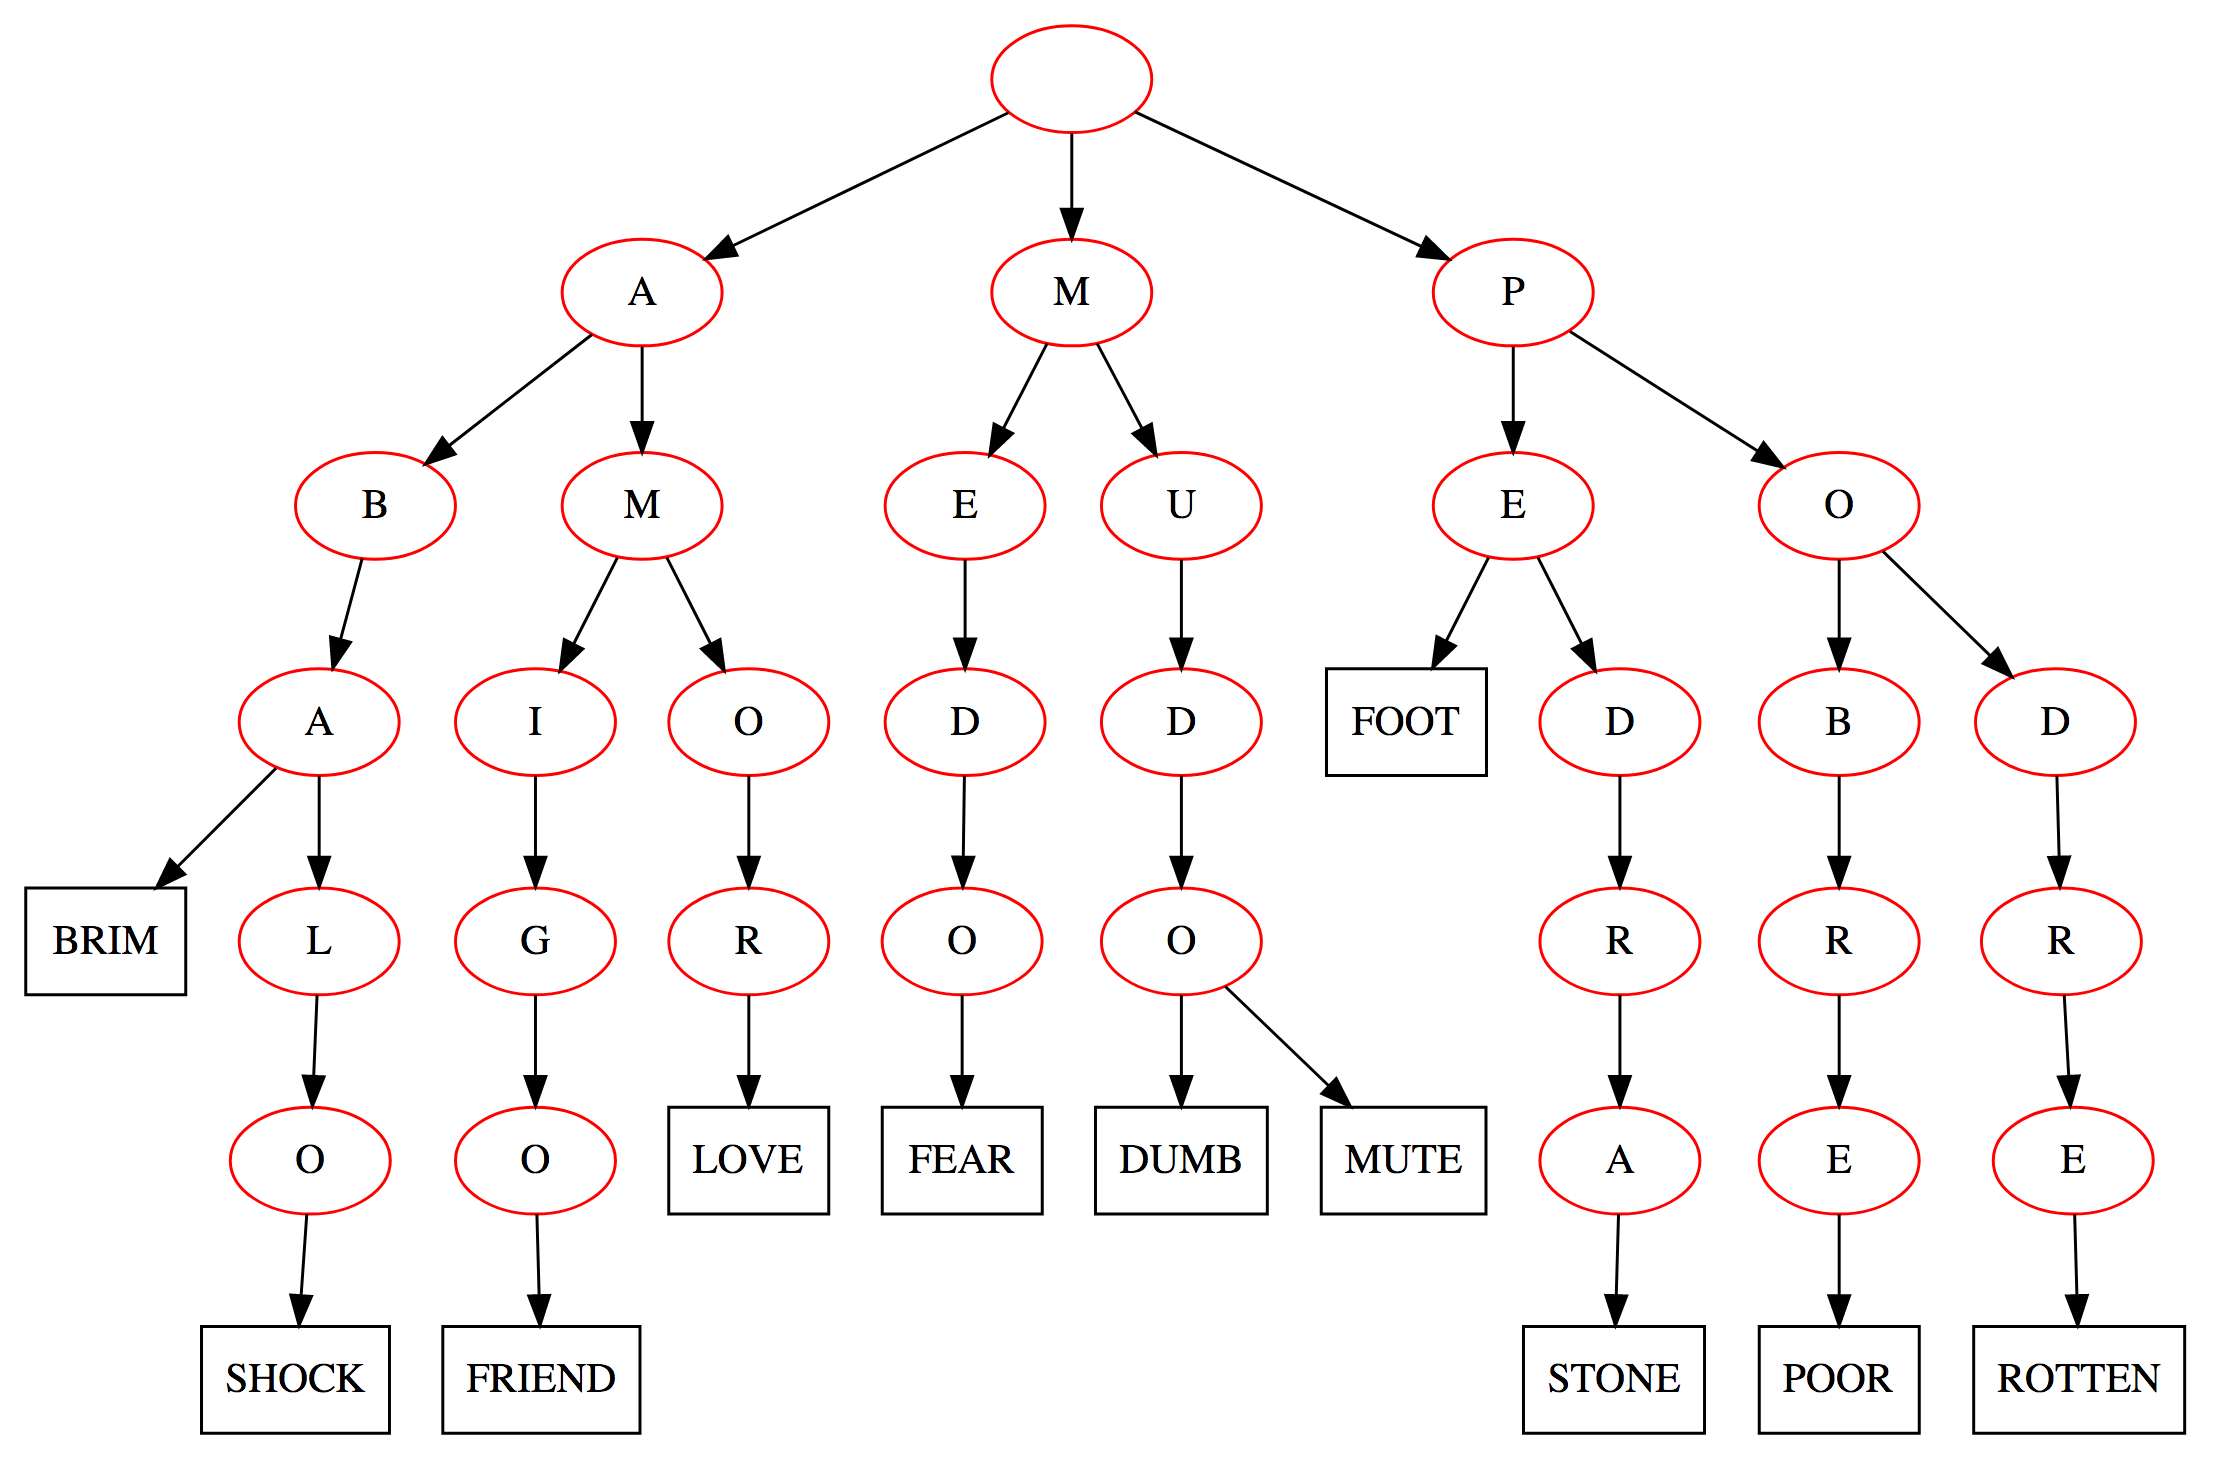
\includegraphics[scale=0.15]{images/dic.png}
    \caption{Representação em memória do dicionário dado para testes.}
    \label{fig:dic}          
    \end{figure}

No anexo \ref{sec:codigo} é dado um dicionário para testes, que corresponde à figura \ref{fig:dic}.
A implementação proposta deverá garantir as seguintes propriedades:
\begin{propriedade}
Se um dicionário estiver normalizado (ver apêndice \ref{sec:codigo}) então
não perdemos informação quando o representamos em memória:
\begin{hscode}\SaveRestoreHook
\column{B}{@{}>{\hspre}l<{\hspost}@{}}%
\column{E}{@{}>{\hspre}l<{\hspost}@{}}%
\>[B]{}\Varid{prop\char95 dic\char95 rep}\;\Varid{x}\mathrel{=}\mathbf{let}\;\Varid{d}\mathrel{=}\Varid{dic\char95 norm}\;\Varid{x}\;\mathbf{in}\;(\Varid{dic\char95 exp}\comp \Varid{dic\char95 imp})\;\Varid{d}\equiv \Varid{d}{}\<[E]%
\ColumnHook
\end{hscode}\resethooks
\end{propriedade}
\begin{propriedade}
Se um significado \ensuremath{\Varid{s}} de uma palavra \ensuremath{\Varid{p}} já existe num dicionário então adicioná-lo
em memória não altera nada:
\begin{hscode}\SaveRestoreHook
\column{B}{@{}>{\hspre}l<{\hspost}@{}}%
\column{4}{@{}>{\hspre}l<{\hspost}@{}}%
\column{E}{@{}>{\hspre}l<{\hspost}@{}}%
\>[B]{}\Varid{prop\char95 dic\char95 red}\;\Varid{p}\;\Varid{s}\;\Varid{d}{}\<[E]%
\\
\>[B]{}\hsindent{4}{}\<[4]%
\>[4]{}\mid \Varid{dic\char95 red}\;\Varid{p}\;\Varid{s}\;\Varid{d}\mathrel{=}\Varid{dic\char95 imp}\;\Varid{d}\equiv \Varid{dic\char95 in}\;\Varid{p}\;\Varid{s}\;(\Varid{dic\char95 imp}\;\Varid{d}){}\<[E]%
\\
\>[B]{}\hsindent{4}{}\<[4]%
\>[4]{}\mid \Varid{otherwise}\mathrel{=}\Conid{True}{}\<[E]%
\ColumnHook
\end{hscode}\resethooks
\end{propriedade}
\begin{propriedade}
A operação \ensuremath{\Varid{dic\char95 rd}} implementa a procura na correspondente exportação do dicionário:
\begin{hscode}\SaveRestoreHook
\column{B}{@{}>{\hspre}l<{\hspost}@{}}%
\column{29}{@{}>{\hspre}l<{\hspost}@{}}%
\column{E}{@{}>{\hspre}l<{\hspost}@{}}%
\>[B]{}\Varid{prop\char95 dic\char95 rd}\;(\Varid{p},\Varid{t})\mathrel{=}\Varid{dic\char95 rd}\;{}\<[29]%
\>[29]{}\Varid{p}\;\Varid{t}\equiv \Varid{lookup}\;\Varid{p}\;(\Varid{dic\char95 exp}\;\Varid{t}){}\<[E]%
\ColumnHook
\end{hscode}\resethooks
\end{propriedade}

\Problema

Árvores binárias (elementos do tipo \BTree) são
    frequentemente usadas no armazenamento e procura de dados, porque
    suportam um vasto conjunto de ferramentas para procuras
    eficientes. Um exemplo de destaque é o caso das
    \href{https://en.wikipedia.org/wiki/Binary_search_tree}{árvores
    binárias de procura}, \emph{i.e.} árvores que seguem o
    princípio de \emph{ordenação}: para todos os nós,
    o filho à esquerda tem um
    valor menor ou igual que o valor no próprio nó; e de forma
     análoga, o filho à direita
    tem um valor maior ou igual que o valor no próprio nó.
    A Figura~\ref{fig:ex} apresenta dois exemplos de árvores binárias de procura.\footnote{
    As imagens foram geradas com recurso à função \ensuremath{\Varid{dotBt}} (disponível
    neste documento). Recomenda-se o
    uso desta função para efeitos de teste e ilustração.}

    \begin{figure}          
    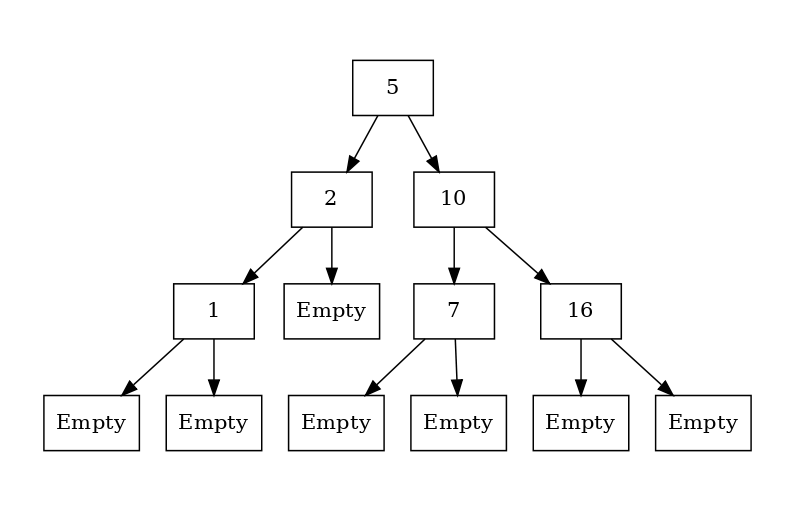
\includegraphics[scale=0.26]{images/example1.png}
    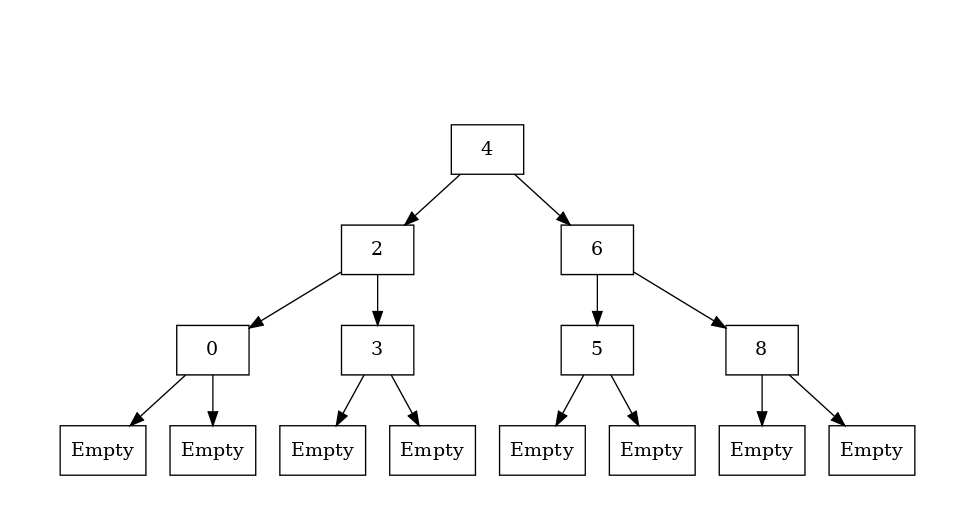
\includegraphics[scale=0.26]{images/example2.png}
    \caption{Duas árvores binárias de procura; a da esquerda vai ser designada
    por $t_1$ e a da direita por $t_2$.}
    \label{fig:ex}          
    \end{figure}
  Note que tais árvores permitem reduzir \emph{significativamente}
  o espaço de procura, dado que ao procurar um valor podemos sempre
  \emph{reduzir a procura a um ramo} ao longo de cada nó visitado. Por
  exemplo, ao procurar o valor $7$ na primeira árvore ($t_1$), sabemos que nos
  podemos restringir ao ramo da direita do nó com o valor $5$ e assim
  sucessivamente. Como complemento a esta explicação, consulte
  também os \href{http://www4.di.uminho.pt/~jno/media/}{vídeos das aulas teóricas} (capítulo `pesquisa binária').

  Para verificar se uma árvore binária está ordenada,
  é útil ter em conta  a seguinte
  propriedade: considere uma árvore binária cuja raíz tem o valor
  $a$, um filho $s_1$ à esquerda e um filho $s_2$ à direita.
  Assuma que os dois filhos estão ordenados; que o elemento
  \emph{mais à direita} de $t_1$ é menor ou igual a $a$; e que o
  elemento \emph{mais à esquerda} de $t_2$ é maior ou igual a $a$.
  Então a árvore binária está ordenada. Dada esta informação,
  implemente as seguintes funções como catamorfismos de árvores binárias.
\begin{hscode}\SaveRestoreHook
\column{B}{@{}>{\hspre}l<{\hspost}@{}}%
\column{E}{@{}>{\hspre}l<{\hspost}@{}}%
\>[B]{}\Varid{maisEsq}\mathbin{::}\fun{BTree} \;\Varid{a}\to \Conid{Maybe}\;\Varid{a}{}\<[E]%
\\
\>[B]{}\Varid{maisDir}\mathbin{::}\fun{BTree} \;\Varid{a}\to \Conid{Maybe}\;\Varid{a}{}\<[E]%
\ColumnHook
\end{hscode}\resethooks
  Seguem alguns exemplos dos resultados que se esperam ao aplicar
  estas funções à árvore da esquerda ($t1$) e à árvore da direita ($t2$)
  da Figura~\ref{fig:ex}.
  \begin{Verbatim}[fontsize=\small]
   *Splay> maisDir t1
    Just 16
   *Splay> maisEsq t1
    Just 1
   *Splay> maisDir t2
    Just 8
   *Splay> maisEsq t2
    Just 0
  \end{Verbatim}
  \begin{propriedade}
  As funções \ensuremath{\Varid{maisEsq}} e \ensuremath{\Varid{maisDir}} são determinadas unicamente
  pela propriedade
\begin{hscode}\SaveRestoreHook
\column{B}{@{}>{\hspre}l<{\hspost}@{}}%
\column{E}{@{}>{\hspre}l<{\hspost}@{}}%
\>[B]{}\Varid{prop\char95 inv}\mathbin{::}\fun{BTree} \;\Conid{String}\to \Conid{Bool}{}\<[E]%
\\
\>[B]{}\Varid{prop\char95 inv}\mathrel{=}\Varid{maisEsq}\equiv\Varid{maisDir}\comp \Varid{invBTree}{}\<[E]%
\ColumnHook
\end{hscode}\resethooks
  \end{propriedade}
  \begin{propriedade}
    O elemento mais à esquerda de uma árvore está presente no ramo da
    esquerda, a não ser que esse ramo esteja vazio:
\begin{hscode}\SaveRestoreHook
\column{B}{@{}>{\hspre}l<{\hspost}@{}}%
\column{E}{@{}>{\hspre}l<{\hspost}@{}}%
\>[B]{}\Varid{propEsq}\;\Conid{Empty}\mathrel{=}\Varid{property}\;\Conid{Discard}{}\<[E]%
\\
\>[B]{}\Varid{propEsq}\;\Varid{x}\mathord{@}(\Conid{Node}\;(\Varid{a},(\Varid{t},\Varid{s})))\mathrel{=}(\Varid{maisEsq}\;\Varid{t})\not\equiv \Conid{Nothing}\Rightarrow(\Varid{maisEsq}\;\Varid{x})\equiv \Varid{maisEsq}\;\Varid{t}{}\<[E]%
\ColumnHook
\end{hscode}\resethooks
\end{propriedade}
  A próxima tarefa deste problema consiste na implementação de uma função
  que insere um novo elemento numa árvore
  binária \emph{preservando} o princípio de ordenação,
\begin{hscode}\SaveRestoreHook
\column{B}{@{}>{\hspre}l<{\hspost}@{}}%
\column{E}{@{}>{\hspre}l<{\hspost}@{}}%
\>[B]{}\Varid{insOrd}\mathbin{::}(\Conid{Ord}\;\Varid{a})\Rightarrow \Varid{a}\to \fun{BTree} \;\Varid{a}\to \fun{BTree} \;\Varid{a}{}\<[E]%
\ColumnHook
\end{hscode}\resethooks
  e de uma função que verifica se uma dada árvore binária está ordenada,
\begin{hscode}\SaveRestoreHook
\column{B}{@{}>{\hspre}l<{\hspost}@{}}%
\column{E}{@{}>{\hspre}l<{\hspost}@{}}%
\>[B]{}\Varid{isOrd}\mathbin{::}(\Conid{Ord}\;\Varid{a})\Rightarrow \fun{BTree} \;\Varid{a}\to \Conid{Bool}{}\<[E]%
\ColumnHook
\end{hscode}\resethooks
Para ambas as funções deve utilizar o que aprendeu sobre \emph{catamorfismos e
recursividade mútua}.

\noindent
\textbf{Sugestão:} Se tiver problemas em implementar
com base em catamorfismos  estas duas últimas
funções, tente implementar (com base em catamorfismos) as funções auxiliares
\begin{hscode}\SaveRestoreHook
\column{B}{@{}>{\hspre}l<{\hspost}@{}}%
\column{E}{@{}>{\hspre}l<{\hspost}@{}}%
\>[B]{}\Varid{insOrd'}\mathbin{::}(\Conid{Ord}\;\Varid{a})\Rightarrow \Varid{a}\to \fun{BTree} \;\Varid{a}\to (\fun{BTree} \;\Varid{a},\fun{BTree} \;\Varid{a}){}\<[E]%
\\
\>[B]{}\Varid{isOrd'}\mathbin{::}(\Conid{Ord}\;\Varid{a})\Rightarrow \fun{BTree} \;\Varid{a}\to (\Conid{Bool},\fun{BTree} \;\Varid{a}){}\<[E]%
\ColumnHook
\end{hscode}\resethooks
tais que
$insOrd' \> x = \langle insOrd \> x, id \rangle$ para todo o elemento $x$
do tipo $a$
e
$isOrd' = \langle isOrd, id \rangle$.
  \begin{propriedade}
   Inserir uma sucessão de elementos numa árvore vazia gera uma árvore
   ordenada.
\begin{hscode}\SaveRestoreHook
\column{B}{@{}>{\hspre}l<{\hspost}@{}}%
\column{E}{@{}>{\hspre}l<{\hspost}@{}}%
\>[B]{}\Varid{prop\char95 ord}\mathbin{::}[\mskip1.5mu \Conid{Int}\mskip1.5mu]\to \Conid{Bool}{}\<[E]%
\\
\>[B]{}\Varid{prop\char95 ord}\mathrel{=}\Varid{isOrd}\comp (\Varid{foldr}\;\Varid{insOrd}\;\Conid{Empty}){}\<[E]%
\ColumnHook
\end{hscode}\resethooks
\end{propriedade}

\smallskip
  \noindent
    As árvores binárias providenciam uma boa maneira de reduzir o espaço
    de procura. Mas podemos fazer ainda melhor: podemos aproximar da
    raíz os elementos da árvore que são mais acedidos, reduzindo assim
    o espaço de procura na \emph{dimensão vertical}\footnote{Note que
    nas árvores de binária de procura a redução é feita na dimensão
    horizontal.}. Esta operação é geralmente
    referida como
    \href{https://en.wikipedia.org/wiki/Splay_tree}{\emph{splaying}} e
    é implementada com base naquilo a que chamamos
    \href{https://en.wikipedia.org/wiki/Tree_rotation}{\emph{rotações à esquerda
    e à direita de uma  árvore}}.

    Intuitivamente, a rotação à direita de uma árvore move todos os
    nós "\emph{uma casa para a sua direita}". Formalmente,
    esta operação define-se da seguinte maneira:
    \begin{enumerate}
       \item Considere uma árvore binária e designe a sua
       raíz pela letra $r$. Se $r$ não tem filhos à esquerda então simplesmente
       retornamos a árvore dada à entrada. Caso contrário,
       \item designe o filho à esquerda pela letra $l$. A árvore
       que vamos retornar tem $l$ na raíz, que mantém o filho à esquerda
       e adopta $r$ como o filho à direita. O orfão (\emph{i.e.} o anterior
       filho à direita de $l$) passa a ser o filho à esquerda de $r$.
    \end{enumerate}
    A rotação à esquerda é definida de forma análoga. As
       Figuras~\ref{exrot:fig} e \ref{exrot2:fig} apresentam dois
       exemplos de rotações à direita. Note que em ambos os casos o
       valor $2$ subiu um nível na árvore correspodente. De facto,
       podemos sempre aplicar uma \emph{sequência} de rotações numa
       árvore de forma a mover um dado nó para a raíz (dando origem
       portanto à referida operação de splaying).

    \begin{figure}
    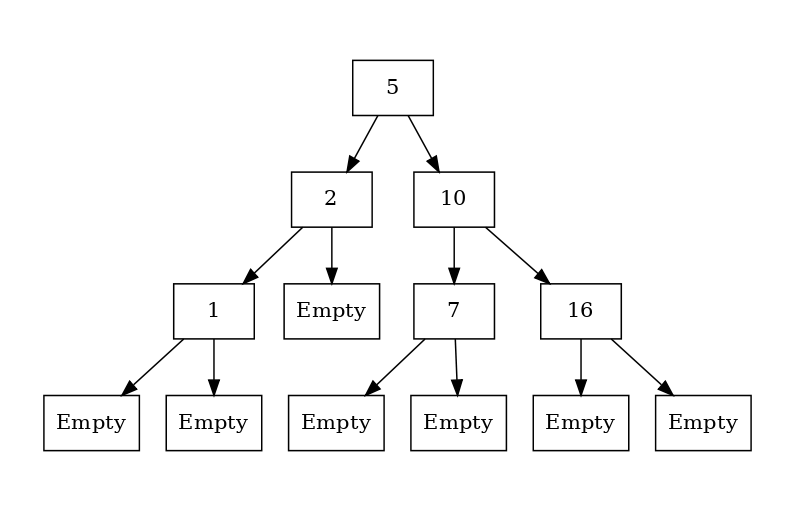
\includegraphics[scale=0.27]{images/example1.png}
    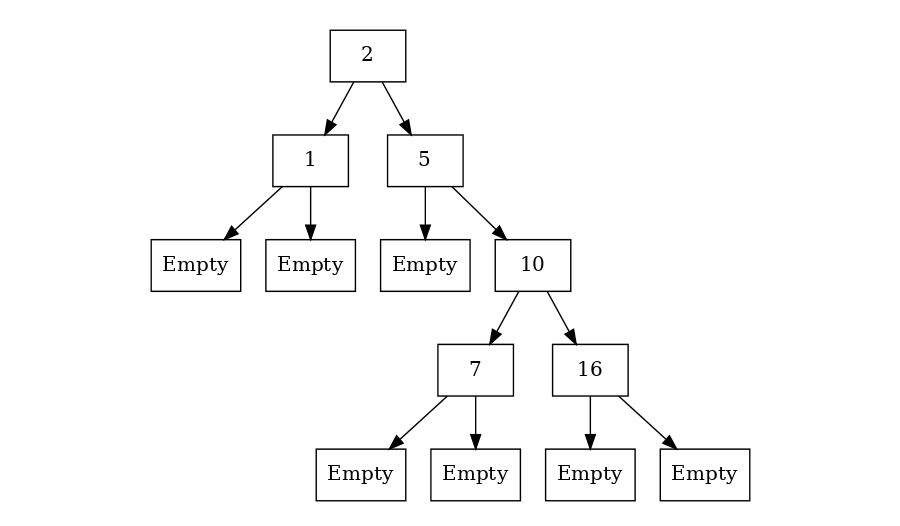
\includegraphics[scale=0.27]{images/example3.png}
    \caption{Exemplo de uma rotação à direita. A árvore da esquerda
    é a árvore original; a árvore da direita representa a rotação à direita
    correspondente.}
    \label{exrot:fig}
    \end{figure}

    \begin{figure}
    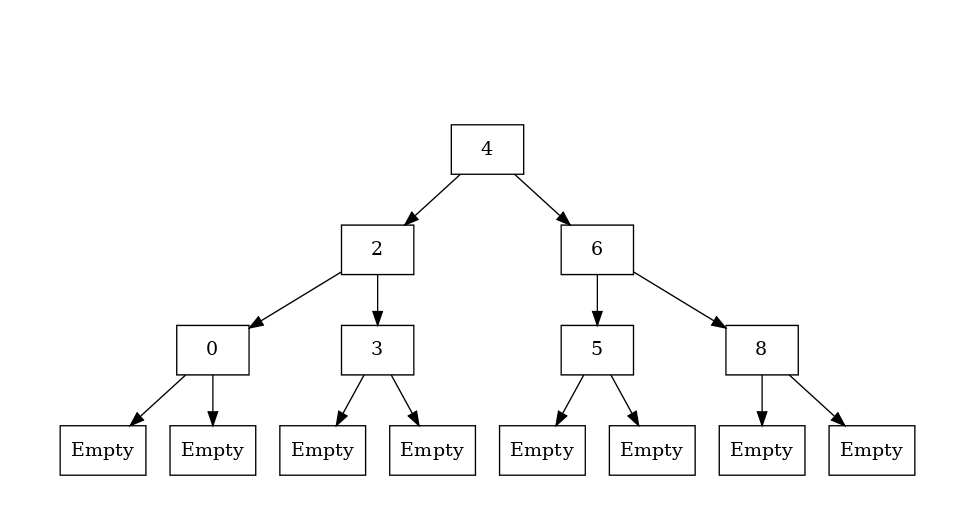
\includegraphics[scale=0.25]{images/example2.png}
    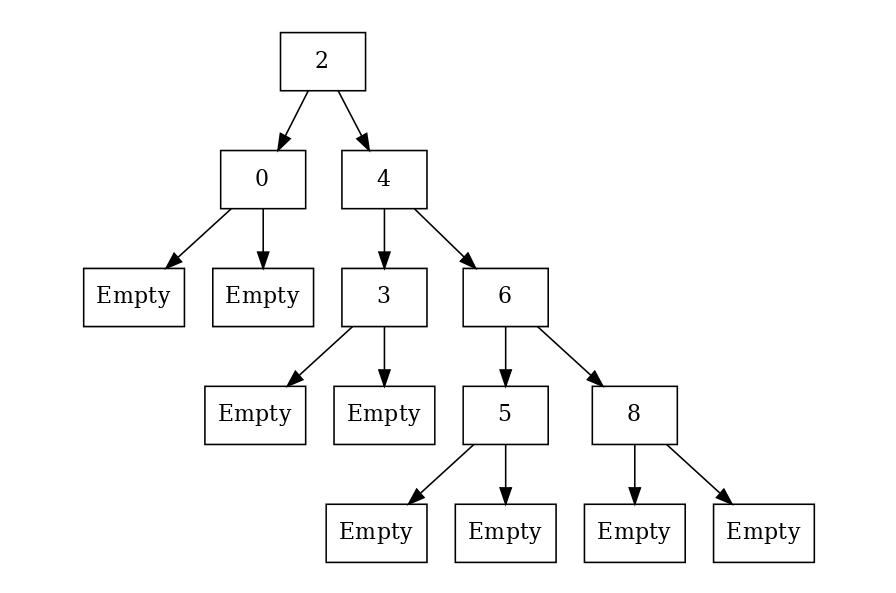
\includegraphics[scale=0.25]{images/example4.png}
    \caption{Exemplo de uma rotação à direita. A árvore da esquerda
    é a árvore original; a árvore da direita representa a rotação à direita
    correspondente.}
    \label{exrot2:fig}
    \end{figure}

    Começe então por implementar as funções   
\begin{hscode}\SaveRestoreHook
\column{B}{@{}>{\hspre}l<{\hspost}@{}}%
\column{E}{@{}>{\hspre}l<{\hspost}@{}}%
\>[B]{}\Varid{rrot}\mathbin{::}\fun{BTree} \;\Varid{a}\to \fun{BTree} \;\Varid{a}{}\<[E]%
\\
\>[B]{}\Varid{lrot}\mathbin{::}\fun{BTree} \;\Varid{a}\to \fun{BTree} \;\Varid{a}{}\<[E]%
\ColumnHook
\end{hscode}\resethooks
    de rotação à direita e à esquerda.
    \begin{propriedade}
       As rotações à esquerda e à direita preservam a ordenação
       das árvores.
\begin{hscode}\SaveRestoreHook
\column{B}{@{}>{\hspre}l<{\hspost}@{}}%
\column{E}{@{}>{\hspre}l<{\hspost}@{}}%
\>[B]{}\Varid{prop\char95 ord\char95 pres\char95 esq}\mathrel{=}\Varid{forAll}\;\Varid{orderedBTree}\;(\Varid{isOrd}\comp \Varid{lrot}){}\<[E]%
\\
\>[B]{}\Varid{prop\char95 ord\char95 pres\char95 dir}\mathrel{=}\Varid{forAll}\;\Varid{orderedBTree}\;(\Varid{isOrd}\comp \Varid{rrot}){}\<[E]%
\ColumnHook
\end{hscode}\resethooks
    \end{propriedade}
De seguida implemente a operação de splaying
\begin{hscode}\SaveRestoreHook
\column{B}{@{}>{\hspre}l<{\hspost}@{}}%
\column{E}{@{}>{\hspre}l<{\hspost}@{}}%
\>[B]{}\Varid{splay}\mathbin{::}[\mskip1.5mu \Conid{Bool}\mskip1.5mu]\to (\fun{BTree} \;\Varid{a}\to \fun{BTree} \;\Varid{a}){}\<[E]%
\ColumnHook
\end{hscode}\resethooks
como um catamorfismo de listas. O argumento \ensuremath{[\mskip1.5mu \Conid{Bool}\mskip1.5mu]}
representa um caminho ao longo de uma árvore, em que o valor \ensuremath{\Conid{True}}
representa "seguir pelo ramo da esquerda" e o valor \ensuremath{\Conid{False}}
representa "seguir pelo ramo da direita". O caminho ao longo de uma árvore serve
para \emph{identificar} unicamente um nó dessa árvore.
\begin{propriedade}
A operação de splay preserva a ordenação de uma árvore.
\begin{hscode}\SaveRestoreHook
\column{B}{@{}>{\hspre}l<{\hspost}@{}}%
\column{E}{@{}>{\hspre}l<{\hspost}@{}}%
\>[B]{}\Varid{prop\char95 ord\char95 pres\char95 splay}\mathbin{::}[\mskip1.5mu \Conid{Bool}\mskip1.5mu]\to \Conid{Property}{}\<[E]%
\\
\>[B]{}\Varid{prop\char95 ord\char95 pres\char95 splay}\;\Varid{path}\mathrel{=}\Varid{forAll}\;\Varid{orderedBTree}\;(\Varid{isOrd}\comp (\Varid{splay}\;\Varid{path})){}\<[E]%
\ColumnHook
\end{hscode}\resethooks
\end{propriedade}

\Problema

\emph{Árvores de decisão binárias} são estruturas de dados usadas na
 área de
 \href{https://www.xoriant.com/blog/product-engineering/decision-trees-machine-learning-algorithm.html}{machine
 learning} para codificar processos de decisão. Geralmente, tais
 árvores são geradas por computadores com base num vasto conjunto de
 dados e reflectem o que o computador "aprendeu" ao processar esses
 mesmos dados. Segue-se um exemplo muito simples de uma árvore de decisão
 binária:

\[
  \xymatrix{ & \text{chuva na ida?} \ar[dl]_{\text{sim}} \ar[dr]^{\text{não}} & &\\
  \text{precisa} & & \text{chuva no regresso?} \ar[dl]^{\text{sim}}
  \ar[dr]^{\text{não}} & \\
  & \text{precisa} & & \text{não precisa}
  }
\]

Esta árvore representa o processo de decisão relativo a ser preciso ou
    não levar um guarda-chuva para uma viagem, dependendo das
    condições climatéricas. Essencialmente, o processo de decisão é
    efectuado ao "percorrer" a árvore, escolhendo o ramo da esquerda ou
    da direita de acordo com a resposta à pergunta correspondente. Por
    exemplo, começando da raiz da árvore, responder \ensuremath{[\mskip1.5mu \text{\ttfamily \char34 não\char34},\text{\ttfamily \char34 não\char34}\mskip1.5mu]}
    leva-nos à decisão \ensuremath{\text{\ttfamily \char34 não~precisa\char34}} e responder \ensuremath{[\mskip1.5mu \text{\ttfamily \char34 não\char34},\text{\ttfamily \char34 sim\char34}\mskip1.5mu]}
    leva-nos à decisão \ensuremath{\text{\ttfamily \char34 precisa\char34}}.

Árvores de decisão binárias podem ser codificadas em \Haskell\ usando
o seguinte tipo de dados:
\begin{hscode}\SaveRestoreHook
\column{B}{@{}>{\hspre}l<{\hspost}@{}}%
\column{E}{@{}>{\hspre}l<{\hspost}@{}}%
\>[B]{}\mathbf{data}\;\Conid{Bdt}\;\Varid{a}\mathrel{=}\Conid{Dec}\;\Varid{a}\mid \Conid{Query}\;(\Conid{String},(\Conid{Bdt}\;\Varid{a},\Conid{Bdt}\;\Varid{a}))\;\mathbf{deriving}\;\Conid{Show}{}\<[E]%
\ColumnHook
\end{hscode}\resethooks

Note que o tipo de dados \ensuremath{\Conid{Bdt}} é parametrizado por um tipo de dados
 \ensuremath{\Varid{a}}.  Isto é necessário, porque as decisões podem ser de diferentes
 tipos: por exemplo, respostas do tipo "sim ou não" (como apresentado
 acima), a escolha de números, ou
 \href{http://jkurokawa.com/2018/02/09/machine-learning-part-ii-decision-trees}{classificações}.

De forma a conseguirmos processar árvores de decisão binárias em \Haskell,
deve, antes de tudo, resolver as seguintes alíneas:
\begin{enumerate}
  \item Definir as funções \ensuremath{\Varid{inBdt}}, \ensuremath{\Varid{outBdt}}, \ensuremath{\Varid{baseBdt}}, \ensuremath{\Varid{cataBdt}}, e \ensuremath{\Varid{anaBdt}}.
  \item Apresentar no relatório o diagrama de \ensuremath{\Varid{anaBdt}}.
\end{enumerate}
Para tomar uma decisão com base numa árvore de decisão binária \ensuremath{\Varid{t}}, o
computador precisa apenas da estrutura de \ensuremath{\Varid{t}} (\emph{i.e.} pode esquecer
a informação nos nós da árvore) e de uma lista de respostas "sim ou não" (para
que possa percorrer a árvore da forma desejada). Implemente então as seguintes
funções na forma de \emph{catamorfismos}:
\begin{enumerate}
\item \ensuremath{\Varid{extLTree}\mathbin{:}\Conid{Bdt}\;\Varid{a}\to \mathsf{LTree}\;\Varid{a}} (esquece a informação presente
nos nós de uma dada árvore de decisão binária).
\begin{propriedade}
  A função \ensuremath{\Varid{extLTree}} preserva as folhas da árvore de origem.
\begin{hscode}\SaveRestoreHook
\column{B}{@{}>{\hspre}l<{\hspost}@{}}%
\column{E}{@{}>{\hspre}l<{\hspost}@{}}%
\>[B]{}\Varid{prop\char95 pres\char95 tips}\mathbin{::}\Conid{Bdt}\;\Conid{Int}\to \Conid{Bool}{}\<[E]%
\\
\>[B]{}\Varid{prop\char95 pres\char95 tips}\mathrel{=}\Varid{tipsBdt}\equiv\Varid{tipsLTree}\comp \Varid{extLTree}{}\<[E]%
\ColumnHook
\end{hscode}\resethooks
\end{propriedade}
\item \ensuremath{\Varid{navLTree}\mathbin{:}\mathsf{LTree}\;\Varid{a}\to ([\mskip1.5mu \Conid{Bool}\mskip1.5mu]\to \mathsf{LTree}\;\Varid{a})} (navega um elemento de
\ensuremath{\mathsf{LTree}}
de acordo com uma sequência de respostas "sim ou não". Esta função deve
ser implementada como um catamorfismo de \ensuremath{\mathsf{LTree}}. Neste contexto,
elementos de \ensuremath{[\mskip1.5mu \Conid{Bool}\mskip1.5mu]} representam sequências de respostas: o valor \ensuremath{\Conid{True}} corresponde a "sim" e portanto a "segue pelo ramo da esquerda"; o valor
\ensuremath{\Conid{False}} corresponde a "não" e portanto a "segue pelo ramo da direita".

Seguem
alguns exemplos dos resultados que se esperam ao aplicar \ensuremath{\Varid{navLTree}} a
\ensuremath{(\Varid{extLTree}\;\Varid{bdtGC})}, em que \ensuremath{\Varid{bdtGC}} é a  àrvore de decisão binária acima descrita,
e a uma
sequência de respostas.
   \begin{Verbatim}[fontsize=\small]
    *ML> navLTree (extLTree bdtGC) []
    Fork (Leaf "Precisa",Fork (Leaf "Precisa",Leaf "N precisa"))
    *ML> navLTree (extLTree bdtGC) [False]
    Fork (Leaf "Precisa",Leaf "N precisa")
    *ML> navLTree (extLTree bdtGC) [False,True]
    Leaf "Precisa"
    *ML> navLTree (extLTree bdtGC) [False,True,True]
    Leaf "Precisa"
    *ML> navLTree (extLTree bdtGC) [False,True,True,True]
    Leaf "Precisa"
   \end{Verbatim}
\end{enumerate}
\begin{propriedade}
  Percorrer uma árvore ao longo de um caminho é equivalente a percorrer
a árvore inversa ao longo do caminho inverso.
\begin{hscode}\SaveRestoreHook
\column{B}{@{}>{\hspre}l<{\hspost}@{}}%
\column{3}{@{}>{\hspre}l<{\hspost}@{}}%
\column{E}{@{}>{\hspre}l<{\hspost}@{}}%
\>[B]{}\Varid{prop\char95 inv\char95 nav}\mathbin{::}\Conid{Bdt}\;\Conid{Int}\to [\mskip1.5mu \Conid{Bool}\mskip1.5mu]\to \Conid{Bool}{}\<[E]%
\\
\>[B]{}\Varid{prop\char95 inv\char95 nav}\;\Varid{t}\;\Varid{l}\mathrel{=}\mathbf{let}\;\Varid{t'}\mathrel{=}\Varid{extLTree}\;\Varid{t}\;\mathbf{in}{}\<[E]%
\\
\>[B]{}\hsindent{3}{}\<[3]%
\>[3]{}\Varid{invLTree}\;(\Varid{navLTree}\;\Varid{t'}\;\Varid{l})\equiv \Varid{navLTree}\;(\Varid{invLTree}\;\Varid{t'})\;(\mathsf{fmap}\;\neg \;\Varid{l}){}\<[E]%
\ColumnHook
\end{hscode}\resethooks
\end{propriedade}
\begin{propriedade}
  Quanto mais longo for o caminho menos alternativas de fim irão existir.
\begin{hscode}\SaveRestoreHook
\column{B}{@{}>{\hspre}l<{\hspost}@{}}%
\column{21}{@{}>{\hspre}l<{\hspost}@{}}%
\column{25}{@{}>{\hspre}l<{\hspost}@{}}%
\column{E}{@{}>{\hspre}l<{\hspost}@{}}%
\>[B]{}\Varid{prop\char95 af}\mathbin{::}\Conid{Bdt}\;\Conid{Int}\to ([\mskip1.5mu \Conid{Bool}\mskip1.5mu],[\mskip1.5mu \Conid{Bool}\mskip1.5mu])\to \Conid{Property}{}\<[E]%
\\
\>[B]{}\Varid{prop\char95 af}\;\Varid{t}\;(\Varid{l1},\Varid{l2})\mathrel{=}\mathbf{let}\;\Varid{t'}\mathrel{=}\Varid{extLTree}\;\Varid{t}{}\<[E]%
\\
\>[B]{}\hsindent{25}{}\<[25]%
\>[25]{}\Varid{f}\mathrel{=}\length \comp \Varid{tipsLTree}\comp (\Varid{navLTree}\;\Varid{t'}){}\<[E]%
\\
\>[B]{}\hsindent{21}{}\<[21]%
\>[21]{}\mathbf{in}\;\Varid{isPrefixOf}\;\Varid{l1}\;\Varid{l2}\Rightarrow(\Varid{f}\;\Varid{l1}\geq \Varid{f}\;\Varid{l2}){}\<[E]%
\ColumnHook
\end{hscode}\resethooks
\end{propriedade}

\Problema

Mónades são functores com propriedades adicionais que nos permitem obter
efeitos especiais em progra\-mação. Por exemplo, a biblioteca \Probability\
oferece um mónade para abordar problemas de probabilidades. Nesta biblioteca,
o conceito de distribuição estatística é captado pelo tipo
\begin{eqnarray}
	\ensuremath{\mathbf{newtype}\;\fun{Dist}\;\Varid{a}\mathrel{=}\Conid{D}\;\{\mskip1.5mu \Varid{unD}\mathbin{::}[\mskip1.5mu (\Varid{a},\Conid{ProbRep})\mskip1.5mu]\mskip1.5mu\}}
	\label{eq:Dist}
\end{eqnarray}
em que \ensuremath{\Conid{ProbRep}} é um real de \ensuremath{\mathrm{0}} a \ensuremath{\mathrm{1}}, equivalente a uma escala de $0$ a
$100 \%$.

Cada par \ensuremath{(\Varid{a},\Varid{p})} numa distribuição \ensuremath{\Varid{d}\mathbin{::}\fun{Dist}\;\Varid{a}} indica que a probabilidade
de \ensuremath{\Varid{a}} é \ensuremath{\Varid{p}}, devendo ser garantida a propriedade de  que todas as probabilidades
de \ensuremath{\Varid{d}} somam $100\%$.
Por exemplo, a seguinte distribuição de classificações por escalões de $A$ a $E$,
\[
\begin{array}{ll}
A & \rule{2mm}{3pt}\ 2\%\\
B & \rule{12mm}{3pt}\ 12\%\\
C & \rule{29mm}{3pt}\ 29\%\\
D & \rule{35mm}{3pt}\ 35\%\\
E & \rule{22mm}{3pt}\ 22\%\\
\end{array}
\]
será representada pela distribuição
\begin{hscode}\SaveRestoreHook
\column{B}{@{}>{\hspre}l<{\hspost}@{}}%
\column{E}{@{}>{\hspre}l<{\hspost}@{}}%
\>[B]{}\Varid{d1}\mathbin{::}\fun{Dist}\;\Conid{Char}{}\<[E]%
\\
\>[B]{}\Varid{d1}\mathrel{=}\Conid{D}\;[\mskip1.5mu (\text{\ttfamily 'A'},\mathrm{0.02}),(\text{\ttfamily 'B'},\mathrm{0.12}),(\text{\ttfamily 'C'},\mathrm{0.29}),(\text{\ttfamily 'D'},\mathrm{0.35}),(\text{\ttfamily 'E'},\mathrm{0.22})\mskip1.5mu]{}\<[E]%
\ColumnHook
\end{hscode}\resethooks
que o \GHCi\ mostrará assim:
\begin{Verbatim}[fontsize=\small]
'D'  35.0%
'C'  29.0%
'E'  22.0%
'B'  12.0%
'A'   2.0%
\end{Verbatim}
É possível definir geradores de distribuições, por exemplo distribuições \emph{uniformes},
\begin{hscode}\SaveRestoreHook
\column{B}{@{}>{\hspre}l<{\hspost}@{}}%
\column{E}{@{}>{\hspre}l<{\hspost}@{}}%
\>[B]{}\Varid{d2}\mathrel{=}\Varid{uniform}\;(\Varid{words}\;\text{\ttfamily \char34 Uma~frase~de~cinco~palavras\char34}){}\<[E]%
\ColumnHook
\end{hscode}\resethooks
isto é
\begin{Verbatim}[fontsize=\small]
     "Uma"  20.0%
   "cinco"  20.0%
      "de"  20.0%
   "frase"  20.0%
"palavras"  20.0%
\end{Verbatim}
distribuição \emph{normais}, eg.\
\begin{hscode}\SaveRestoreHook
\column{B}{@{}>{\hspre}l<{\hspost}@{}}%
\column{E}{@{}>{\hspre}l<{\hspost}@{}}%
\>[B]{}\Varid{d3}\mathrel{=}\Varid{normal}\;[\mskip1.5mu \mathrm{10}\mathinner{\ldotp\ldotp}\mathrm{20}\mskip1.5mu]{}\<[E]%
\ColumnHook
\end{hscode}\resethooks
etc.\footnote{Para mais detalhes ver o código fonte de \Probability, que é uma adaptação da
biblioteca \PFP\ (``Probabilistic Functional Programming''). Para quem quiser souber mais
recomenda-se a leitura do artigo \cite{EK06}.}
\ensuremath{\fun{Dist}} forma um \textbf{mónade} cuja unidade é \ensuremath{\Varid{return}\;\Varid{a}\mathrel{=}\Conid{D}\;[\mskip1.5mu (\Varid{a},\mathrm{1})\mskip1.5mu]} e cuja composição de Kleisli
é (simplificando a notação)
\begin{hscode}\SaveRestoreHook
\column{B}{@{}>{\hspre}l<{\hspost}@{}}%
\column{3}{@{}>{\hspre}l<{\hspost}@{}}%
\column{E}{@{}>{\hspre}l<{\hspost}@{}}%
\>[3]{}(\Varid{f}\kcomp \Varid{g})\;\Varid{a}\mathrel{=}[\mskip1.5mu (\Varid{y},\Varid{q}\mathbin{*}\Varid{p})\mid (\Varid{x},\Varid{p})\leftarrow \Varid{g}\;\Varid{a},(\Varid{y},\Varid{q})\leftarrow \Varid{f}\;\Varid{x}\mskip1.5mu]{}\<[E]%
\ColumnHook
\end{hscode}\resethooks
em que \ensuremath{\Varid{g}\mathbin{:}\Conid{A}\to \fun{Dist}\;\mathit B} e \ensuremath{\Varid{f}\mathbin{:}\mathit B\to \fun{Dist}\;\mathit C} são funções \textbf{monádicas} que representam
\emph{computações probabilísticas}.
Este mónade é adequado à resolução de problemas de
 \emph{probabilidades e estatística} usando programação funcional, de
 forma elegante e como caso particular da programação
 monádica. Vamos estudar a aplicação
 deste mónade ao exercício anterior, tendo em conta o facto de que nem
 sempre podemos responder com 100\% de certeza a perguntas presentes
 em árvores de decisão.


Considere a seguinte situação: a Anita vai
 trabalhar no dia seguinte
e quer saber se precisa de levar guarda-chuva.  Na verdade,
 ela tem autocarro de porta de casa até ao trabalho, e portanto
 as condições meteorológicas não são muito significativas; a não ser
 que seja segunda-feira...Às segundas é dia de feira e o autocarro vai
 sempre lotado! Nesses dias, ela prefere fazer a pé o caminho de casa
 ao trabalho, o que a obriga a levar guarda-chuva (nos dias de
 chuva). Abaixo está apresentada a árvore de decisão respectiva a este problema.

 \[
     \xymatrix{
     && \text{2a-feira?} \ar[dl]_{\text{sim}} \ar[dr]^{\text{não}} & \\
     & \text{chuva na ida?} \ar[dl]_{\text{sim}} \ar[dr]^{\text{não}}
      && \text{não precisa} \\
     \text{precisa} && \text{chuva no regresso?}
    \ar[dl]_{\text{sim}} \ar[dr]^{\text{não}} & \\
     &\text{precisa} && \text{não precisa}
     }
  \]

Assuma que a Anita não sabe em que dia está, e que a previsão da
   chuva para a ida é de 80\% enquanto que a previsão de chuva para o
   regresso é de 60\%. \emph{A Anita deve
  levar guarda-chuva?}
  Para responder a esta questão, iremos tirar partido do que se aprendeu
  no exercício anterior. De facto, a maior diferença é que agora as
  respostas ("sim" ou "não") são dadas na forma de uma distribuição sobre o tipo de dados
  \ensuremath{\Conid{Bool}}. Implemente como um catamorfismo de \ensuremath{\mathsf{LTree}} a função
\begin{hscode}\SaveRestoreHook
\column{B}{@{}>{\hspre}l<{\hspost}@{}}%
\column{E}{@{}>{\hspre}l<{\hspost}@{}}%
\>[B]{}\Varid{bnavLTree}\mathbin{::}\mathsf{LTree}\;\Varid{a}\to ((\fun{BTree} \;\Conid{Bool})\to \mathsf{LTree}\;\Varid{a}){}\<[E]%
\ColumnHook
\end{hscode}\resethooks
que percorre uma árvore dado um caminho, \emph{não} do tipo \ensuremath{[\mskip1.5mu \Conid{Bool}\mskip1.5mu]}, mas
do tipo \ensuremath{\fun{BTree} \;\Conid{Bool}}. O tipo \ensuremath{\fun{BTree} \;\Conid{Bool}} é necessário
na presença de incerteza, porque neste contexto não sabemos sempre
       qual a próxima pergunta a responder. Teremos portanto
que ter resposta para todas as perguntas na árvore de decisão.

Seguem alguns exemplos dos resultados que se esperam
       ao aplicar \ensuremath{\Varid{bnavLTree}} a \ensuremath{(\Varid{extLTree}\;\Varid{anita})}, em que \ensuremath{\Varid{anita}} é a
       árvore de decisão acima descrita, e a uma árvore
      binária de respostas.
     \begin{Verbatim}[fontsize=\small]
      *ML> bnavLTree (extLTree anita) (Node(True, (Empty,Empty)))
      Fork (Leaf "Precisa",Fork (Leaf "Precisa",Leaf "N precisa"))
      *ML> bnavLTree (extLTree anita) (Node(True, (Node(True,(Empty,Empty)),Empty)))
      Leaf "Precisa"
      *ML> bnavLTree (extLTree anita) (Node(False, (Empty,Empty)))
      Leaf "N precisa"
     \end{Verbatim}
Por fim, implemente como um catamorfismo de \ensuremath{\mathsf{LTree}} a função
\begin{hscode}\SaveRestoreHook
\column{B}{@{}>{\hspre}l<{\hspost}@{}}%
\column{E}{@{}>{\hspre}l<{\hspost}@{}}%
\>[B]{}\Varid{pbnavLTree}\mathbin{::}\mathsf{LTree}\;\Varid{a}\to ((\fun{BTree} \;(\fun{Dist}\;\Conid{Bool}))\to \fun{Dist}\;(\mathsf{LTree}\;\Varid{a})){}\<[E]%
\ColumnHook
\end{hscode}\resethooks
que deverá consiste na "monadificação" da função \ensuremath{\Varid{bnavLTree}} via a mónade das
probabilidades. Use esta última implementação para responder se a Anita deve
levar guarda-chuva ou não dada a situação acima descrita.
\Problema

Os \truchet{mosaicos de Truchet} são padrões que se obtêm gerando aleatoriamente
combinações bidimensionais de ladrilhos básicos. Os que se mostram na figura
\ref{fig:tiles} são conhecidos por ladrilhos de Truchet-Smith.
A figura \ref{fig:truchet} mostra um exemplo de mosaico produzido por uma
combinação aleatória de 10x10 ladrilhos \ensuremath{\Varid{a}} e \ensuremath{\Varid{b}} (cf.\ figura
\ref{fig:tiles}).

Neste problema pretende-se programar a geração aleatória de mosaicos de
Truchet-Smith usando o mónade \random{Random} e a biblioteca \gloss{Gloss}
para produção do resultado. Para uniformização das respostas, deverão ser
seguidas as seguintes condições:
\begin{itemize}
\item	Cada ladrilho deverá ter as dimensões 80x80
\item	O programa deverá gerar mosaicos de quaisquer dimensões, mas deverá ser apresentado como figura no relatório o mosaico de 10x10 ladrilhos.
\item	Valorizar-se-ão respostas elegantes e com menos linhas de código \Haskell.
\end{itemize} 
No anexo \ref{sec:codigo} é dada uma implementação da operação de permuta aleatória de uma lista que pode ser útil para resolver este exercício.

    \begin{figure}\centering
    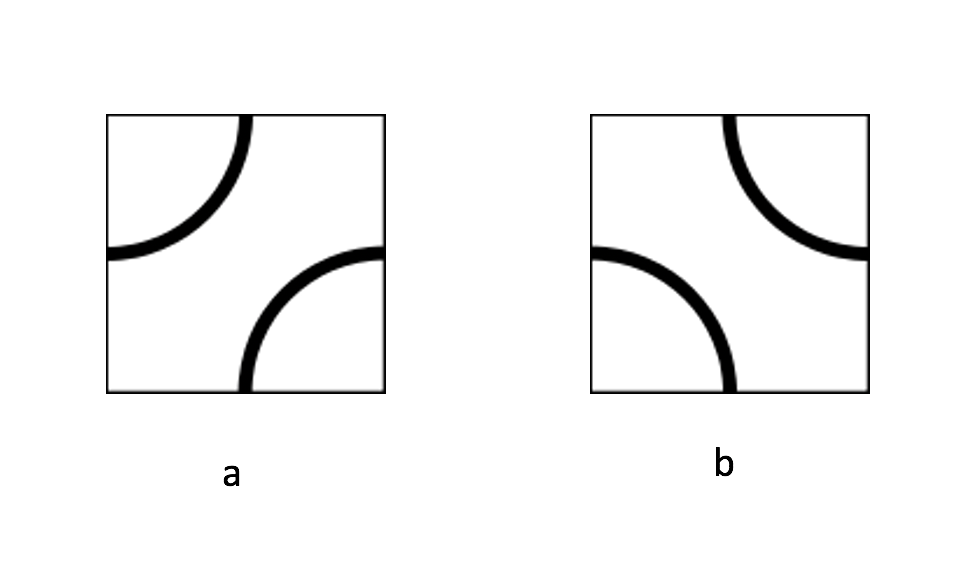
\includegraphics[scale=0.20]{images/tiles.png}
    \caption{Os dois ladrilhos de Truchet-Smith.}
    \label{fig:tiles}
    \end{figure}

    \begin{figure}\centering
    
\includegraphics[scale=0.20]{images/truchet.png}
    \caption{Um mosaico de Truchet-Smith.}
    \label{fig:truchet}
    \end{figure}

%----------------- Programa, bibliotecas e código auxiliar --------------------%

\newpage

\part*{Anexos}

\appendix

\section{Como exprimir cálculos e diagramas em LaTeX/lhs2tex}
Estudar o texto fonte deste trabalho para obter o efeito:\footnote{Exemplos tirados de \cite{Ol18}.} 
\begin{eqnarray*}
\start
	\ensuremath{\Varid{id}\mathrel{=}\conj{\Varid{f}}{\Varid{g}}}
%
\just\equiv{ universal property }
%
        \ensuremath{\begin{lcbr}\p1\comp \Varid{id}\mathrel{=}\Varid{f}\\\p2\comp \Varid{id}\mathrel{=}\Varid{g}\end{lcbr}}
%
\just\equiv{ identity }
%
        \ensuremath{\begin{lcbr}\p1\mathrel{=}\Varid{f}\\\p2\mathrel{=}\Varid{g}\end{lcbr}}
\qed
\end{eqnarray*}

Os diagramas podem ser produzidos recorrendo à \emph{package} \LaTeX\ 
\href{https://ctan.org/pkg/xymatrix}{xymatrix}, por exemplo: 
\begin{eqnarray*}
\xymatrix@C=2cm{
    \ensuremath{\N_0}
           \ar[d]_-{\ensuremath{\cata{\Varid{g}}}}
&
    \ensuremath{\mathrm{1}\mathbin{+}\N_0}
           \ar[d]^{\ensuremath{\Varid{id}\mathbin{+}\cata{\Varid{g}}}}
           \ar[l]_-{\ensuremath{\mathsf{in}}}
\\
     \ensuremath{\mathit B}
&
     \ensuremath{\mathrm{1}\mathbin{+}\mathit B}
           \ar[l]^-{\ensuremath{\Varid{g}}}
}
\end{eqnarray*}


\section{Código fornecido}\label{sec:codigo}

\subsection*{Problema 1}
Função de representação de um dicionário:
\begin{hscode}\SaveRestoreHook
\column{B}{@{}>{\hspre}l<{\hspost}@{}}%
\column{32}{@{}>{\hspre}l<{\hspost}@{}}%
\column{E}{@{}>{\hspre}l<{\hspost}@{}}%
\>[B]{}\Varid{dic\char95 imp}\mathbin{::}[\mskip1.5mu (\Conid{String},[\mskip1.5mu \Conid{String}\mskip1.5mu])\mskip1.5mu]\to \Conid{Dict}{}\<[E]%
\\
\>[B]{}\Varid{dic\char95 imp}\mathrel{=}\Conid{Term}\;\text{\ttfamily \char34 \char34}\comp \map \;(\Varid{bmap}\;{}\<[32]%
\>[32]{}\Varid{id}\;\Varid{singl})\comp \Varid{untar}\comp \Varid{discollect}{}\<[E]%
\ColumnHook
\end{hscode}\resethooks
onde
\begin{hscode}\SaveRestoreHook
\column{B}{@{}>{\hspre}l<{\hspost}@{}}%
\column{E}{@{}>{\hspre}l<{\hspost}@{}}%
\>[B]{}\mathbf{type}\;\Conid{Dict}\mathrel{=}\Conid{Exp}\;\Conid{String}\;\Conid{String}{}\<[E]%
\ColumnHook
\end{hscode}\resethooks
Dicionário para testes:
\begin{hscode}\SaveRestoreHook
\column{B}{@{}>{\hspre}l<{\hspost}@{}}%
\column{6}{@{}>{\hspre}l<{\hspost}@{}}%
\column{8}{@{}>{\hspre}l<{\hspost}@{}}%
\column{E}{@{}>{\hspre}l<{\hspost}@{}}%
\>[B]{}\Varid{d}\mathbin{::}[\mskip1.5mu (\Conid{String},[\mskip1.5mu \Conid{String}\mskip1.5mu])\mskip1.5mu]{}\<[E]%
\\
\>[B]{}\Varid{d}\mathrel{=}{}\<[6]%
\>[6]{}[\mskip1.5mu (\text{\ttfamily \char34 ABA\char34},[\mskip1.5mu \text{\ttfamily \char34 BRIM\char34}\mskip1.5mu]),{}\<[E]%
\\
\>[6]{}\hsindent{2}{}\<[8]%
\>[8]{}(\text{\ttfamily \char34 ABALO\char34},[\mskip1.5mu \text{\ttfamily \char34 SHOCK\char34}\mskip1.5mu]),{}\<[E]%
\\
\>[6]{}\hsindent{2}{}\<[8]%
\>[8]{}(\text{\ttfamily \char34 AMIGO\char34},[\mskip1.5mu \text{\ttfamily \char34 FRIEND\char34}\mskip1.5mu]),{}\<[E]%
\\
\>[6]{}\hsindent{2}{}\<[8]%
\>[8]{}(\text{\ttfamily \char34 AMOR\char34},[\mskip1.5mu \text{\ttfamily \char34 LOVE\char34}\mskip1.5mu]),{}\<[E]%
\\
\>[6]{}\hsindent{2}{}\<[8]%
\>[8]{}(\text{\ttfamily \char34 MEDO\char34},[\mskip1.5mu \text{\ttfamily \char34 FEAR\char34}\mskip1.5mu]),{}\<[E]%
\\
\>[6]{}\hsindent{2}{}\<[8]%
\>[8]{}(\text{\ttfamily \char34 MUDO\char34},[\mskip1.5mu \text{\ttfamily \char34 DUMB\char34},\text{\ttfamily \char34 MUTE\char34}\mskip1.5mu]),{}\<[E]%
\\
\>[6]{}\hsindent{2}{}\<[8]%
\>[8]{}(\text{\ttfamily \char34 PE\char34},[\mskip1.5mu \text{\ttfamily \char34 FOOT\char34}\mskip1.5mu]),{}\<[E]%
\\
\>[6]{}\hsindent{2}{}\<[8]%
\>[8]{}(\text{\ttfamily \char34 PEDRA\char34},[\mskip1.5mu \text{\ttfamily \char34 STONE\char34}\mskip1.5mu]),{}\<[E]%
\\
\>[6]{}\hsindent{2}{}\<[8]%
\>[8]{}(\text{\ttfamily \char34 POBRE\char34},[\mskip1.5mu \text{\ttfamily \char34 POOR\char34}\mskip1.5mu]),{}\<[E]%
\\
\>[6]{}\hsindent{2}{}\<[8]%
\>[8]{}(\text{\ttfamily \char34 PODRE\char34},[\mskip1.5mu \text{\ttfamily \char34 ROTTEN\char34}\mskip1.5mu])\mskip1.5mu]{}\<[E]%
\ColumnHook
\end{hscode}\resethooks
Normalização de um dicionário (remoção de entradas vazias):
\begin{hscode}\SaveRestoreHook
\column{B}{@{}>{\hspre}l<{\hspost}@{}}%
\column{4}{@{}>{\hspre}l<{\hspost}@{}}%
\column{E}{@{}>{\hspre}l<{\hspost}@{}}%
\>[B]{}\Varid{dic\char95 norm}\mathrel{=}\Varid{collect}\comp \Varid{filter}\;\Varid{p}\comp \Varid{discollect}\;\mathbf{where}{}\<[E]%
\\
\>[B]{}\hsindent{4}{}\<[4]%
\>[4]{}\Varid{p}\;(\Varid{a},\Varid{b})\mathrel{=}\Varid{a}\mathbin{>}\text{\ttfamily \char34 \char34}\mathrel{\wedge}\Varid{b}\mathbin{>}\text{\ttfamily \char34 \char34}{}\<[E]%
\ColumnHook
\end{hscode}\resethooks
Teste de redundância de um significado \ensuremath{\Varid{s}} para uma palavra \ensuremath{\Varid{p}}:
\begin{hscode}\SaveRestoreHook
\column{B}{@{}>{\hspre}l<{\hspost}@{}}%
\column{E}{@{}>{\hspre}l<{\hspost}@{}}%
\>[B]{}\Varid{dic\char95 red}\;\Varid{p}\;\Varid{s}\;\Varid{d}\mathrel{=}(\Varid{p},\Varid{s})\in \Varid{discollect}\;\Varid{d}{}\<[E]%
\ColumnHook
\end{hscode}\resethooks

\subsection*{Problema 2}

Árvores usadas no texto:
\begin{hscode}\SaveRestoreHook
\column{B}{@{}>{\hspre}l<{\hspost}@{}}%
\column{E}{@{}>{\hspre}l<{\hspost}@{}}%
\>[B]{}\Varid{emp}\;\Varid{x}\mathrel{=}\Conid{Node}\;(\Varid{x},(\Conid{Empty},\Conid{Empty})){}\<[E]%
\\[\blanklineskip]%
\>[B]{}\Varid{t7}\mathrel{=}\Varid{emp}\;\mathrm{7}{}\<[E]%
\\
\>[B]{}\Varid{t16}\mathrel{=}\Varid{emp}\;\mathrm{16}{}\<[E]%
\\
\>[B]{}\Varid{t7\char95 10\char95 16}\mathrel{=}\Conid{Node}\;(\mathrm{10},(\Varid{t7},\Varid{t16})){}\<[E]%
\\
\>[B]{}\Varid{t1\char95 2\char95 nil}\mathrel{=}\Conid{Node}\;(\mathrm{2},(\Varid{emp}\;\mathrm{1},\Conid{Empty})){}\<[E]%
\\
\>[B]{}\Varid{t'}\mathrel{=}\Conid{Node}\;(\mathrm{5},(\Varid{t1\char95 2\char95 nil},\Varid{t7\char95 10\char95 16})){}\<[E]%
\\[\blanklineskip]%
\>[B]{}\Varid{t0\char95 2\char95 1}\mathrel{=}\Conid{Node}\;(\mathrm{2},(\Varid{emp}\;\mathrm{0},\Varid{emp}\;\mathrm{3})){}\<[E]%
\\
\>[B]{}\Varid{t5\char95 6\char95 8}\mathrel{=}\Conid{Node}\;(\mathrm{6},(\Varid{emp}\;\mathrm{5},\Varid{emp}\;\mathrm{8})){}\<[E]%
\\
\>[B]{}\Varid{t2}\mathrel{=}\Conid{Node}\;(\mathrm{4},(\Varid{t0\char95 2\char95 1},\Varid{t5\char95 6\char95 8})){}\<[E]%
\\[\blanklineskip]%
\>[B]{}\Varid{dotBt}\mathbin{::}(\Conid{Show}\;\Varid{a})\Rightarrow \fun{BTree} \;\Varid{a}\to \fun{IO}\;\Conid{ExitCode}{}\<[E]%
\\
\>[B]{}\Varid{dotBt}\mathrel{=}\Varid{dotpict}\comp \Varid{bmap}\;\Conid{Just}\;\Conid{Just}\comp \Varid{cBTree2Exp}\comp (\mathsf{fmap}\;\Varid{show}){}\<[E]%
\ColumnHook
\end{hscode}\resethooks

\subsection*{Problema 3}
Funções usadas para efeitos de teste:
\begin{hscode}\SaveRestoreHook
\column{B}{@{}>{\hspre}l<{\hspost}@{}}%
\column{E}{@{}>{\hspre}l<{\hspost}@{}}%
\>[B]{}\Varid{tipsBdt}\mathbin{::}\Conid{Bdt}\;\Varid{a}\to [\mskip1.5mu \Varid{a}\mskip1.5mu]{}\<[E]%
\\
\>[B]{}\Varid{tipsBdt}\mathrel{=}\Varid{cataBdt}\;\alt{\Varid{singl}}{\uncurry{(\plus )}\comp \p2}{}\<[E]%
\\
\>[B]{}\Varid{tipsLTree}\mathrel{=}\Varid{tips}{}\<[E]%
\ColumnHook
\end{hscode}\resethooks

\subsection*{Problema 5}
Função de permutação aleatória de uma lista:
\begin{hscode}\SaveRestoreHook
\column{B}{@{}>{\hspre}l<{\hspost}@{}}%
\column{7}{@{}>{\hspre}l<{\hspost}@{}}%
\column{E}{@{}>{\hspre}l<{\hspost}@{}}%
\>[B]{}\Varid{permuta}\;[\mskip1.5mu \mskip1.5mu]\mathrel{=}\Varid{return}\;[\mskip1.5mu \mskip1.5mu]{}\<[E]%
\\
\>[B]{}\Varid{permuta}\;\Varid{x}\mathrel{=}\mathbf{do}\;\{\mskip1.5mu (\Varid{h},\Varid{t})\leftarrow \Varid{getR}\;\Varid{x};\Varid{t'}\leftarrow \Varid{permuta}\;\Varid{t};\Varid{return}\;(\Varid{h}\mathbin{:}\Varid{t'})\mskip1.5mu\}\;\mathbf{where}{}\<[E]%
\\
\>[B]{}\hsindent{7}{}\<[7]%
\>[7]{}\Varid{getR}\;\Varid{x}\mathrel{=}\mathbf{do}\;\{\mskip1.5mu \Varid{i}\leftarrow \Varid{getStdRandom}\;(\Varid{randomR}\;(\mathrm{0},\length \;\Varid{x}\mathbin{-}\mathrm{1}));\Varid{return}\;(\Varid{x}\mathbin{!!}\Varid{i},\Varid{retira}\;\Varid{i}\;\Varid{x})\mskip1.5mu\}{}\<[E]%
\\
\>[B]{}\hsindent{7}{}\<[7]%
\>[7]{}\Varid{retira}\;\Varid{i}\;\Varid{x}\mathrel{=}\Varid{take}\;\Varid{i}\;\Varid{x}\plus \Varid{drop}\;(\Varid{i}\mathbin{+}\mathrm{1})\;\Varid{x}{}\<[E]%
\ColumnHook
\end{hscode}\resethooks

\subsection*{QuickCheck}
Código para geração de testes:
\begin{hscode}\SaveRestoreHook
\column{B}{@{}>{\hspre}l<{\hspost}@{}}%
\column{5}{@{}>{\hspre}l<{\hspost}@{}}%
\column{15}{@{}>{\hspre}l<{\hspost}@{}}%
\column{17}{@{}>{\hspre}l<{\hspost}@{}}%
\column{23}{@{}>{\hspre}c<{\hspost}@{}}%
\column{23E}{@{}l@{}}%
\column{26}{@{}>{\hspre}l<{\hspost}@{}}%
\column{30}{@{}>{\hspre}l<{\hspost}@{}}%
\column{62}{@{}>{\hspre}l<{\hspost}@{}}%
\column{E}{@{}>{\hspre}l<{\hspost}@{}}%
\>[B]{}\mathbf{instance}\;\Conid{Arbitrary}\;\Varid{a}\Rightarrow \Conid{Arbitrary}\;(\fun{BTree} \;\Varid{a})\;\mathbf{where}{}\<[E]%
\\
\>[B]{}\hsindent{5}{}\<[5]%
\>[5]{}\Varid{arbitrary}\mathrel{=}\Varid{sized}\;\Varid{genbt}\;{}\<[30]%
\>[30]{}\mathbf{where}{}\<[E]%
\\
\>[5]{}\hsindent{10}{}\<[15]%
\>[15]{}\Varid{genbt}\;\mathrm{0}\mathrel{=}\Varid{return}\;(\Varid{inBTree}\mathbin{\$}i_1\;()){}\<[E]%
\\
\>[5]{}\hsindent{10}{}\<[15]%
\>[15]{}\Varid{genbt}\;\Varid{n}\mathrel{=}\Varid{oneof}\;[\mskip1.5mu (\Varid{liftM2}\mathbin{\$}\Varid{curry}\;(\Varid{inBTree}\comp i_2)){}\<[E]%
\\
\>[15]{}\hsindent{2}{}\<[17]%
\>[17]{}\Varid{\Conid{QuickCheck}.arbitrary}\;(\Varid{liftM2}\;(,)\;(\Varid{genbt}\;(\Varid{n}\mathbin{-}\mathrm{1}))\;(\Varid{genbt}\;(\Varid{n}\mathbin{-}\mathrm{1}))),{}\<[E]%
\\
\>[15]{}\hsindent{2}{}\<[17]%
\>[17]{}(\Varid{liftM2}\mathbin{\$}\Varid{curry}\;(\Varid{inBTree}\comp i_2)){}\<[E]%
\\
\>[15]{}\hsindent{2}{}\<[17]%
\>[17]{}\Varid{\Conid{QuickCheck}.arbitrary}\;(\Varid{liftM2}\;(,)\;(\Varid{genbt}\;(\Varid{n}\mathbin{-}\mathrm{1}))\;(\Varid{genbt}\;\mathrm{0})),{}\<[E]%
\\
\>[15]{}\hsindent{2}{}\<[17]%
\>[17]{}(\Varid{liftM2}\mathbin{\$}\Varid{curry}\;(\Varid{inBTree}\comp i_2)){}\<[E]%
\\
\>[15]{}\hsindent{2}{}\<[17]%
\>[17]{}\Varid{\Conid{QuickCheck}.arbitrary}\;(\Varid{liftM2}\;(,)\;(\Varid{genbt}\;\mathrm{0})\;(\Varid{genbt}\;(\Varid{n}\mathbin{-}\mathrm{1})))\mskip1.5mu]{}\<[E]%
\\[\blanklineskip]%
\>[B]{}\mathbf{instance}\;(\Conid{Arbitrary}\;\Varid{v},\Conid{Arbitrary}\;\Varid{o})\Rightarrow \Conid{Arbitrary}\;(\Conid{Exp}\;\Varid{v}\;\Varid{o})\;\mathbf{where}{}\<[E]%
\\
\>[B]{}\hsindent{5}{}\<[5]%
\>[5]{}\Varid{arbitrary}\mathrel{=}(\Varid{genExp}\;\mathrm{10})\;{}\<[30]%
\>[30]{}\mathbf{where}{}\<[E]%
\\
\>[5]{}\hsindent{10}{}\<[15]%
\>[15]{}\Varid{genExp}\;\mathrm{0}\mathrel{=}\Varid{liftM}\;(\Varid{inExp}\comp i_1)\;\Varid{\Conid{QuickCheck}.arbitrary}{}\<[E]%
\\
\>[5]{}\hsindent{10}{}\<[15]%
\>[15]{}\Varid{genExp}\;\Varid{n}\mathrel{=}\Varid{oneof}\;[\mskip1.5mu \Varid{liftM}\;(\Varid{inExp}\comp i_2\comp (\lambda \Varid{a}\to (\Varid{a},[\mskip1.5mu \mskip1.5mu])))\;\Varid{\Conid{QuickCheck}.arbitrary},{}\<[E]%
\\
\>[15]{}\hsindent{11}{}\<[26]%
\>[26]{}\Varid{liftM}\;(\Varid{inExp}\comp i_1)\;\Varid{\Conid{QuickCheck}.arbitrary},{}\<[E]%
\\
\>[15]{}\hsindent{11}{}\<[26]%
\>[26]{}\Varid{liftM}\;(\Varid{inExp}\comp i_2\comp (\lambda (\Varid{a},(\Varid{b},\Varid{c}))\to (\Varid{a},[\mskip1.5mu \Varid{b},\Varid{c}\mskip1.5mu]))){}\<[E]%
\\
\>[15]{}\hsindent{11}{}\<[26]%
\>[26]{}\mathbin{\$}(\Varid{liftM2}\;(,)\;\Varid{\Conid{QuickCheck}.arbitrary}\;(\Varid{liftM2}\;(,){}\<[E]%
\\
\>[26]{}\hsindent{36}{}\<[62]%
\>[62]{}(\Varid{genExp}\;(\Varid{n}\mathbin{-}\mathrm{1}))\;(\Varid{genExp}\;(\Varid{n}\mathbin{-}\mathrm{1})))),{}\<[E]%
\\
\>[15]{}\hsindent{11}{}\<[26]%
\>[26]{}\Varid{liftM}\;(\Varid{inExp}\comp i_2\comp (\lambda (\Varid{a},(\Varid{b},\Varid{c},\Varid{d}))\to (\Varid{a},[\mskip1.5mu \Varid{b},\Varid{c},\Varid{d}\mskip1.5mu]))){}\<[E]%
\\
\>[15]{}\hsindent{11}{}\<[26]%
\>[26]{}\mathbin{\$}(\Varid{liftM2}\;(,)\;\Varid{\Conid{QuickCheck}.arbitrary}\;(\Varid{liftM3}\;(,,){}\<[E]%
\\
\>[26]{}\hsindent{36}{}\<[62]%
\>[62]{}(\Varid{genExp}\;(\Varid{n}\mathbin{-}\mathrm{1}))\;(\Varid{genExp}\;(\Varid{n}\mathbin{-}\mathrm{1}))\;(\Varid{genExp}\;(\Varid{n}\mathbin{-}\mathrm{1})))){}\<[E]%
\\
\>[15]{}\hsindent{8}{}\<[23]%
\>[23]{}\mskip1.5mu]{}\<[23E]%
\\[\blanklineskip]%
\>[B]{}\Varid{orderedBTree}\mathbin{::}\Conid{Gen}\;(\fun{BTree} \;\Conid{Int}){}\<[E]%
\\
\>[B]{}\Varid{orderedBTree}\mathrel{=}\Varid{liftM}\;(\Varid{foldr}\;\Varid{insOrd}\;\Conid{Empty})\;(\Varid{\Conid{QuickCheck}.arbitrary}\mathbin{::}\Conid{Gen}\;[\mskip1.5mu \Conid{Int}\mskip1.5mu]){}\<[E]%
\\[\blanklineskip]%
\>[B]{}\mathbf{instance}\;(\Conid{Arbitrary}\;\Varid{a})\Rightarrow \Conid{Arbitrary}\;(\Conid{Bdt}\;\Varid{a})\;\mathbf{where}{}\<[E]%
\\
\>[B]{}\hsindent{5}{}\<[5]%
\>[5]{}\Varid{arbitrary}\mathrel{=}\Varid{sized}\;\Varid{genbt}\;{}\<[30]%
\>[30]{}\mathbf{where}{}\<[E]%
\\
\>[5]{}\hsindent{10}{}\<[15]%
\>[15]{}\Varid{genbt}\;\mathrm{0}\mathrel{=}\Varid{liftM}\;\Conid{Dec}\;\Varid{\Conid{QuickCheck}.arbitrary}{}\<[E]%
\\
\>[5]{}\hsindent{10}{}\<[15]%
\>[15]{}\Varid{genbt}\;\Varid{n}\mathrel{=}\Varid{oneof}\;[\mskip1.5mu (\Varid{liftM2}\mathbin{\$}\Varid{curry}\;\Conid{Query}){}\<[E]%
\\
\>[15]{}\hsindent{2}{}\<[17]%
\>[17]{}\Varid{\Conid{QuickCheck}.arbitrary}\;(\Varid{liftM2}\;(,)\;(\Varid{genbt}\;(\Varid{n}\mathbin{-}\mathrm{1}))\;(\Varid{genbt}\;(\Varid{n}\mathbin{-}\mathrm{1}))),{}\<[E]%
\\
\>[15]{}\hsindent{2}{}\<[17]%
\>[17]{}(\Varid{liftM2}\mathbin{\$}\Varid{curry}\;(\Conid{Query})){}\<[E]%
\\
\>[15]{}\hsindent{2}{}\<[17]%
\>[17]{}\Varid{\Conid{QuickCheck}.arbitrary}\;(\Varid{liftM2}\;(,)\;(\Varid{genbt}\;(\Varid{n}\mathbin{-}\mathrm{1}))\;(\Varid{genbt}\;\mathrm{0})),{}\<[E]%
\\
\>[15]{}\hsindent{2}{}\<[17]%
\>[17]{}(\Varid{liftM2}\mathbin{\$}\Varid{curry}\;(\Conid{Query})){}\<[E]%
\\
\>[15]{}\hsindent{2}{}\<[17]%
\>[17]{}\Varid{\Conid{QuickCheck}.arbitrary}\;(\Varid{liftM2}\;(,)\;(\Varid{genbt}\;\mathrm{0})\;(\Varid{genbt}\;(\Varid{n}\mathbin{-}\mathrm{1})))\mskip1.5mu]{}\<[E]%
\ColumnHook
\end{hscode}\resethooks

\subsection*{Outras funções auxiliares}
%----------------- Outras definições auxiliares -------------------------------------------%
Lógicas:
\begin{hscode}\SaveRestoreHook
\column{B}{@{}>{\hspre}l<{\hspost}@{}}%
\column{E}{@{}>{\hspre}l<{\hspost}@{}}%
\>[B]{}\mathbf{infixr}\;\mathrm{0}\Rightarrow{}\<[E]%
\\
\>[B]{}(\Rightarrow)\mathbin{::}(\Conid{Testable}\;\Varid{prop})\Rightarrow (\Varid{a}\to \Conid{Bool})\to (\Varid{a}\to \Varid{prop})\to \Varid{a}\to \Conid{Property}{}\<[E]%
\\
\>[B]{}\Varid{p}\Rightarrow\Varid{f}\mathrel{=}\lambda \Varid{a}\to \Varid{p}\;\Varid{a}\Rightarrow\Varid{f}\;\Varid{a}{}\<[E]%
\\[\blanklineskip]%
\>[B]{}\mathbf{infixr}\;\mathrm{0}\Leftrightarrow{}\<[E]%
\\
\>[B]{}(\Leftrightarrow)\mathbin{::}(\Varid{a}\to \Conid{Bool})\to (\Varid{a}\to \Conid{Bool})\to \Varid{a}\to \Conid{Property}{}\<[E]%
\\
\>[B]{}\Varid{p}\Leftrightarrow\Varid{f}\mathrel{=}\lambda \Varid{a}\to (\Varid{p}\;\Varid{a}\Rightarrow\Varid{property}\;(\Varid{f}\;\Varid{a}))\mathbin{.\&\&.}(\Varid{f}\;\Varid{a}\Rightarrow\Varid{property}\;(\Varid{p}\;\Varid{a})){}\<[E]%
\\[\blanklineskip]%
\>[B]{}\mathbf{infixr}\;\mathrm{4}\equiv{}\<[E]%
\\
\>[B]{}(\equiv)\mathbin{::}\Conid{Eq}\;\Varid{b}\Rightarrow (\Varid{a}\to \Varid{b})\to (\Varid{a}\to \Varid{b})\to (\Varid{a}\to \Conid{Bool}){}\<[E]%
\\
\>[B]{}\Varid{f}\equiv\Varid{g}\mathrel{=}\lambda \Varid{a}\to \Varid{f}\;\Varid{a}\equiv \Varid{g}\;\Varid{a}{}\<[E]%
\\[\blanklineskip]%
\>[B]{}\mathbf{infixr}\;\mathrm{4}\leq{}\<[E]%
\\
\>[B]{}(\leq)\mathbin{::}\Conid{Ord}\;\Varid{b}\Rightarrow (\Varid{a}\to \Varid{b})\to (\Varid{a}\to \Varid{b})\to (\Varid{a}\to \Conid{Bool}){}\<[E]%
\\
\>[B]{}\Varid{f}\leq\Varid{g}\mathrel{=}\lambda \Varid{a}\to \Varid{f}\;\Varid{a}\leq \Varid{g}\;\Varid{a}{}\<[E]%
\\[\blanklineskip]%
\>[B]{}\mathbf{infixr}\;\mathrm{4}\wedge{}\<[E]%
\\
\>[B]{}(\wedge)\mathbin{::}(\Varid{a}\to \Conid{Bool})\to (\Varid{a}\to \Conid{Bool})\to (\Varid{a}\to \Conid{Bool}){}\<[E]%
\\
\>[B]{}\Varid{f}\wedge\Varid{g}\mathrel{=}\lambda \Varid{a}\to ((\Varid{f}\;\Varid{a})\mathrel{\wedge}(\Varid{g}\;\Varid{a})){}\<[E]%
\ColumnHook
\end{hscode}\resethooks
Compilação e execução dentro do interpretador:\footnote{Pode ser útil em testes
envolvendo \gloss{Gloss}. Nesse caso, o teste em causa deve fazer parte de uma função
\ensuremath{\Varid{main}}.}
\begin{hscode}\SaveRestoreHook
\column{B}{@{}>{\hspre}l<{\hspost}@{}}%
\column{E}{@{}>{\hspre}l<{\hspost}@{}}%
\>[B]{}\Varid{run}\mathrel{=}\mathbf{do}\;\{\mskip1.5mu \Varid{system}\;\text{\ttfamily \char34 ghc~cp1920t\char34};\Varid{system}\;\text{\ttfamily \char34 ./cp1920t\char34}\mskip1.5mu\}{}\<[E]%
\ColumnHook
\end{hscode}\resethooks

%----------------- Soluções dos alunos -----------------------------------------%

\section{Soluções dos alunos}\label{sec:resolucao}
Os alunos devem colocar neste anexo as suas soluções aos exercícios
propostos, de acordo com o "layout" que se fornece. Não podem ser
alterados os nomes ou tipos das funções dadas, mas pode ser adicionado texto e/ou 
outras funções auxiliares que sejam necessárias.

\subsection*{Problema 1}

A função discollect abaixo apresentada tira partido da utilização de \\ensuremath{\Varid{de}\;\Varid{modo}\;\Varid{a}\;\Varid{preencher}\;\Varid{cada}\;\Varid{par}\;\Varid{retornado}\;\Varid{com}\;\Varid{o}\;\Varid{respetivo}\;\Varid{valor}\comp \lambda \Varid{begin}\;\{\mskip1.5mu \Varid{code}\mskip1.5mu\}\;\Varid{discollect}\mathbin{::}(\Conid{Ord}\;\Varid{b},\Conid{Ord}\;\Varid{a})\Rightarrow [\mskip1.5mu (\Varid{b},[\mskip1.5mu \Varid{a}\mskip1.5mu])\mskip1.5mu]\to [\mskip1.5mu (\Varid{b},\Varid{a})\mskip1.5mu]\;\Varid{discollect}\;\Varid{d}\mathrel{=}\Varid{\Conid{Cp}.cond}\;\Varid{null}\;\Varid{nil}\;(\mathbf{do}\;\{\mskip1.5mu (\Varid{a},\Varid{x})\leftarrow \Varid{head};\Varid{return}\;([\mskip1.5mu (\Varid{a},\Varid{b})} b <- x]++(discollect . tail) d) }) d
\end{code}

A função de exportação do dicionário usa a ja implementada função collect após a função tar ter retornadoa lista com pares entre a palavra em português e uma lista de possíveis traduções desta.

\begin{hscode}\SaveRestoreHook
\column{B}{@{}>{\hspre}l<{\hspost}@{}}%
\column{E}{@{}>{\hspre}l<{\hspost}@{}}%
\>[B]{}\Varid{dic\char95 exp}\mathbin{::}\Conid{Dict}\to [\mskip1.5mu (\Conid{String},[\mskip1.5mu \Conid{String}\mskip1.5mu])\mskip1.5mu]{}\<[E]%
\\
\>[B]{}\Varid{dic\char95 exp}\mathrel{=}\Varid{collect}\comp \Varid{tar}{}\<[E]%
\ColumnHook
\end{hscode}\resethooks

Como foi dito em cima aqui se encontra a função tar que utiliza como gene uma função que terá como input duas alternativas sendo elas o Var e o Term, logo o gene tem de ser um either. 
Sabendo isso temos apenas de encontrar os seus constituintes g1 e g2.
O constituinte g1 será aplicado ao resultado de outExp . (Var v), tendo o seu retorno de ser uma lsta com apenas um par em que o primeiro constituinte seria "" e o segundo seria a palavra traduzida a qual chegamos(v).
O constituinte g2 será aplicado a (id >< map {\ensuremath{\Varid{cataExp}\;\Varid{g}}} ) . outExp . (Term v d), a partir disto facilmente chegamos a conclusão que g2 será aplicado a (v,k) onde k é uma lista do tipo que temos de retornar e são os pares de traduções que se formam a partir daquele termo v, logo tudo o que temos de fazer é inserir v no inicio do primeiro membro de cada um dos pares da lista k concatenada,
daí ficamos com g2 (v,k) = map ((v++) >< id) (concat k)

\begin{hscode}\SaveRestoreHook
\column{B}{@{}>{\hspre}l<{\hspost}@{}}%
\column{3}{@{}>{\hspre}l<{\hspost}@{}}%
\column{5}{@{}>{\hspre}l<{\hspost}@{}}%
\column{9}{@{}>{\hspre}l<{\hspost}@{}}%
\column{15}{@{}>{\hspre}l<{\hspost}@{}}%
\column{31}{@{}>{\hspre}l<{\hspost}@{}}%
\column{40}{@{}>{\hspre}l<{\hspost}@{}}%
\column{52}{@{}>{\hspre}l<{\hspost}@{}}%
\column{E}{@{}>{\hspre}l<{\hspost}@{}}%
\>[B]{}\Varid{tar}\mathrel{=}\Varid{cataExp}\;\Varid{g}\;\mathbf{where}{}\<[E]%
\\
\>[B]{}\hsindent{3}{}\<[3]%
\>[3]{}\Varid{g}\mathrel{=}\alt{\Varid{g1}}{\Varid{g2}}\;\mathbf{where}{}\<[E]%
\\
\>[3]{}\hsindent{2}{}\<[5]%
\>[5]{}\Varid{g1}\;\Varid{s}\mathrel{=}[\mskip1.5mu (\text{\ttfamily \char34 \char34},\Varid{s})\mskip1.5mu]{}\<[E]%
\\
\>[3]{}\hsindent{2}{}\<[5]%
\>[5]{}\Varid{g2}\;(\Varid{o},\Varid{l})\mathrel{=}\map \;((\Varid{o}\plus )\times\Varid{id})\;(\Varid{concat}\;\Varid{l}){}\<[E]%
\\[\blanklineskip]%
\>[B]{}\Varid{dic\char95 rd}\mathrel{=}\Varid{cataList}\;\alt{\underline{\Varid{g1}}}{\Varid{g2}}{}\<[E]%
\\
\>[B]{}\hsindent{3}{}\<[3]%
\>[3]{}\mathbf{where}\;\Varid{g1}\;(\Conid{Var}\;\Varid{v})\mathrel{=}\Conid{Just}\;[\mskip1.5mu \Varid{v}\mskip1.5mu]{}\<[E]%
\\
\>[3]{}\hsindent{6}{}\<[9]%
\>[9]{}\Varid{g1}\;(\Conid{Term}\;\Varid{o}\;\Varid{l})\mathrel{=}\Conid{Nothing}{}\<[E]%
\\
\>[3]{}\hsindent{6}{}\<[9]%
\>[9]{}\Varid{g2}\;(\Varid{a},\Varid{g2t})\;(\Conid{Term}\;\Varid{o}\;\Varid{l})\mid \Varid{o}\equiv \text{\ttfamily \char34 \char34}\mathrel{=}\Varid{auxSequence}\;(\map \;(\Varid{g2}\;(\Varid{a},\Varid{g2t}))\;\Varid{l}){}\<[E]%
\\
\>[9]{}\hsindent{22}{}\<[31]%
\>[31]{}\mid \Varid{o}\equiv [\mskip1.5mu \Varid{a}\mskip1.5mu]\mathrel{=}\Varid{auxSequence}\;[\mskip1.5mu \Varid{b}\mid \Varid{b}\leftarrow (\map \;\Varid{g2t}\;\Varid{l}),\Conid{Nothing}\not\equiv \Varid{b}\mskip1.5mu]{}\<[E]%
\\
\>[9]{}\hsindent{22}{}\<[31]%
\>[31]{}\mid \Varid{otherwise}\mathrel{=}\Conid{Nothing}{}\<[E]%
\\
\>[3]{}\hsindent{6}{}\<[9]%
\>[9]{}\Varid{g2}\;\anonymous \;(\Conid{Var}\;\Varid{v})\mathrel{=}\Conid{Nothing}{}\<[E]%
\\[\blanklineskip]%
\>[B]{}\Varid{auxSequence}\mathbin{::}[\mskip1.5mu \Conid{Maybe}\;[\mskip1.5mu \Conid{String}\mskip1.5mu]\mskip1.5mu]\to \Conid{Maybe}\;[\mskip1.5mu \Conid{String}\mskip1.5mu]{}\<[E]%
\\
\>[B]{}\Varid{auxSequence}\mathrel{=}\Varid{cataList}\;\alt{\Varid{g1}}{\Varid{g2}}{}\<[E]%
\\
\>[B]{}\hsindent{3}{}\<[3]%
\>[3]{}\mathbf{where}\;\Varid{g1}\mathrel{=}\Varid{nothing}{}\<[E]%
\\
\>[3]{}\hsindent{6}{}\<[9]%
\>[9]{}\Varid{g2}\;(\Conid{Just}\;\Varid{a},\Conid{Just}\;\Varid{t})\mathrel{=}\Conid{Just}\;(\Varid{a}\plus \Varid{t}){}\<[E]%
\\
\>[3]{}\hsindent{6}{}\<[9]%
\>[9]{}\Varid{g2}\;(\Conid{Nothing},\Conid{Nothing})\mathrel{=}\Conid{Nothing}{}\<[E]%
\\
\>[3]{}\hsindent{6}{}\<[9]%
\>[9]{}\Varid{g2}\;(\Conid{Just}\;\Varid{a},\Conid{Nothing})\mathrel{=}\Conid{Just}\;\Varid{a}{}\<[E]%
\\
\>[3]{}\hsindent{6}{}\<[9]%
\>[9]{}\Varid{g2}\;(\Conid{Nothing},\Conid{Just}\;\Varid{a})\mathrel{=}\Conid{Just}\;\Varid{a}{}\<[E]%
\\[\blanklineskip]%
\>[B]{}\Varid{dic\char95 in}\;\Varid{p}\;\Varid{s}\;(\Conid{Term}\;\text{\ttfamily \char34 \char34}\;\Varid{v})\mathrel{=}\Conid{Term}\;\text{\ttfamily \char34 \char34}\;(\Varid{hyloList}\;(\Varid{conquerFunction}\;\Varid{s})\;(\Varid{divideFunction})\;(\Varid{p},\Varid{v})){}\<[E]%
\\[\blanklineskip]%
\>[B]{}\Varid{divideFunction}\mathbin{::}(\Conid{String},[\mskip1.5mu \Conid{Dict}\mskip1.5mu])\to ()+([\mskip1.5mu \Conid{Dict}\mskip1.5mu]+(\Conid{Char},[\mskip1.5mu \Conid{Dict}\mskip1.5mu]),(\Conid{String},[\mskip1.5mu \Conid{Dict}\mskip1.5mu])){}\<[E]%
\\
\>[B]{}\Varid{divideFunction}\;(\text{\ttfamily \char34 \char34},[\mskip1.5mu \mskip1.5mu])\mathrel{=}i_1\;(){}\<[E]%
\\
\>[B]{}\Varid{divideFunction}\;((\Varid{h}\mathbin{:}\Varid{t}),[\mskip1.5mu \mskip1.5mu])\mathrel{=}i_2\;((i_2\;(\Varid{h},[\mskip1.5mu \mskip1.5mu])),(\Varid{t},[\mskip1.5mu \mskip1.5mu])){}\<[E]%
\\
\>[B]{}\Varid{divideFunction}\;(\text{\ttfamily \char34 \char34},\Varid{d})\mathrel{=}i_2\;(i_1\;\Varid{d},(\text{\ttfamily \char34 \char34},[\mskip1.5mu \mskip1.5mu])){}\<[E]%
\\
\>[B]{}\Varid{divideFunction}\;((\Varid{h}\mathbin{:}\Varid{t}),((\Conid{Term}\;\Varid{k}\;\Varid{v})\mathbin{:}\Varid{ds}))\mid \Varid{k}\equiv [\mskip1.5mu \Varid{h}\mskip1.5mu]\mathrel{=}{}\<[52]%
\>[52]{}i_2\;(i_2\;(\Varid{h},\Varid{ds}),(\Varid{t},\Varid{v})){}\<[E]%
\\
\>[B]{}\hsindent{40}{}\<[40]%
\>[40]{}\mid \Varid{otherwise}\mathrel{=}(\alt{i_1\comp \Varid{id}}{i_2\comp (\alt{i_1\comp ((\Conid{Term}\;\Varid{k}\;\Varid{v})\mathbin{:})}{i_2\comp (\Varid{id}\times((\Conid{Term}\;\Varid{k}\;\Varid{v})\mathbin{:}))}\times\Varid{id})}\comp \Varid{divideFunction})\;((\Varid{h}\mathbin{:}\Varid{t}),\Varid{ds}){}\<[E]%
\\
\>[B]{}\Varid{divideFunction}\;((\Varid{h}\mathbin{:}\Varid{t}),(\Varid{d}\mathbin{:}\Varid{ds}))\mathrel{=}(\alt{i_1\comp \Varid{id}}{i_2\comp (\alt{i_1\comp (\Varid{d}\mathbin{:})}{i_2\comp (\Varid{id}\times(\Varid{d}\mathbin{:}))}\times\Varid{id})}\comp \Varid{divideFunction})\;((\Varid{h}\mathbin{:}\Varid{t}),\Varid{ds}){}\<[E]%
\\[\blanklineskip]%
\>[B]{}\Varid{conquerFunction}\mathbin{::}\Conid{String}\to ()+([\mskip1.5mu \Conid{Dict}\mskip1.5mu]+(\Conid{Char},[\mskip1.5mu \Conid{Dict}\mskip1.5mu]),[\mskip1.5mu \Conid{Dict}\mskip1.5mu])\to [\mskip1.5mu \Conid{Dict}\mskip1.5mu]{}\<[E]%
\\
\>[B]{}\Varid{conquerFunction}\;\Varid{t}\;\Varid{l}\mathrel{=}\alt{\underline{[\mskip1.5mu \Conid{Var}\;\Varid{t}\mskip1.5mu]}}{\uncurry{(\Varid{cFaux}\;\Varid{t})}\comp \Varid{swap}}\;\Varid{l}{}\<[E]%
\\[\blanklineskip]%
\>[B]{}\Varid{cFaux}\mathbin{::}\Conid{String}\to [\mskip1.5mu \Conid{Dict}\mskip1.5mu]\to ([\mskip1.5mu \Conid{Dict}\mskip1.5mu]+(\Conid{Char},[\mskip1.5mu \Conid{Dict}\mskip1.5mu]))\to [\mskip1.5mu \Conid{Dict}\mskip1.5mu]{}\<[E]%
\\
\>[B]{}\Varid{cFaux}\;\Varid{t}\;\Varid{l}\mathrel{=}\alt{\Varid{tt1}\;\Varid{t}\;\Varid{l}}{\Varid{tt2}\;\Varid{t}\;\Varid{l}}{}\<[E]%
\\
\>[B]{}\hsindent{9}{}\<[9]%
\>[9]{}\mathbf{where}\;\Varid{tt1}\;\Varid{t}\;\Varid{k}\;\Varid{d}\mathrel{=}(\Conid{Var}\;\Varid{t})\mathbin{:}\Varid{d}{}\<[E]%
\\
\>[9]{}\hsindent{6}{}\<[15]%
\>[15]{}\Varid{tt2}\;\Varid{t}\;\Varid{k}\;(\Varid{l},\Varid{r})\mathrel{=}\Varid{r}\plus [\mskip1.5mu \Conid{Term}\;[\mskip1.5mu \Varid{l}\mskip1.5mu]\;\Varid{k}\mskip1.5mu]{}\<[E]%
\ColumnHook
\end{hscode}\resethooks

\subsection*{Problema 2}


Para a resolução das funções maisDir e maisEsq utilizamos as várias regras aprendidas em Cálculo de Programas para obter a estrutura de g, que seria um either de g1 e g2.
O constituinte g1 seria aplicado ao resultado de out . (Empty) gerando logicamente Nothing pois uma árvore vazia não tem elementos logo não tem Máximo nem mínimo.
O constituinte g2 seria aplicado ao resultado de (id >< ( {\ensuremath{\Varid{cataBTree}\;\Varid{g}}} >< {\ensuremath{\Varid{cataBTree}\;\Varid{g}}})) .out .(Node a (t1,t2)) simplificando iria ser aplicado a (a,(r1,r2)) sendo r1 = {\ensuremath{\Varid{cataBtree}\;\Varid{g}}} e r2 = {\ensuremath{\Varid{cataBTree}\;\Varid{g}}} o que consoante o elemento que queriamos nos retorna o que está abaixo representado.

\begin{hscode}\SaveRestoreHook
\column{B}{@{}>{\hspre}l<{\hspost}@{}}%
\column{3}{@{}>{\hspre}l<{\hspost}@{}}%
\column{5}{@{}>{\hspre}l<{\hspost}@{}}%
\column{E}{@{}>{\hspre}l<{\hspost}@{}}%
\>[B]{}\Varid{maisDir}\mathrel{=}\Varid{cataBTree}\;\Varid{g}\;\mathbf{where}{}\<[E]%
\\
\>[B]{}\hsindent{3}{}\<[3]%
\>[3]{}\Varid{g}\mathrel{=}\alt{\Varid{g1}}{\Varid{g2}}\;\mathbf{where}{}\<[E]%
\\
\>[3]{}\hsindent{2}{}\<[5]%
\>[5]{}\Varid{g1}\mathrel{=}\Varid{nothing}{}\<[E]%
\\
\>[3]{}\hsindent{2}{}\<[5]%
\>[5]{}\Varid{g2}\;(\Varid{a},(\Varid{t1},\Conid{Nothing}))\mathrel{=}\Conid{Just}\;\Varid{a}{}\<[E]%
\\
\>[3]{}\hsindent{2}{}\<[5]%
\>[5]{}\Varid{g2}\;(\Varid{a},(\Varid{t1},\Varid{t2}))\mathrel{=}\Varid{t2}{}\<[E]%
\\[\blanklineskip]%
\>[B]{}\Varid{maisEsq}\mathrel{=}\Varid{cataBTree}\;\Varid{g}\;\mathbf{where}{}\<[E]%
\\
\>[B]{}\hsindent{3}{}\<[3]%
\>[3]{}\Varid{g}\mathrel{=}\alt{\Varid{g1}}{\Varid{g2}}\;\mathbf{where}{}\<[E]%
\\
\>[3]{}\hsindent{2}{}\<[5]%
\>[5]{}\Varid{g1}\mathrel{=}\Varid{nothing}{}\<[E]%
\\
\>[3]{}\hsindent{2}{}\<[5]%
\>[5]{}\Varid{g2}\;(\Varid{a},(\Conid{Nothing},\Varid{t2}))\mathrel{=}\Conid{Just}\;\Varid{a}{}\<[E]%
\\
\>[3]{}\hsindent{2}{}\<[5]%
\>[5]{}\Varid{g2}\;(\Varid{a},(\Varid{t1},\Varid{t2}))\mathrel{=}\Varid{t1}{}\<[E]%
\ColumnHook
\end{hscode}\resethooks

Para a resolução da função abaixo recorremos ao enunciado, à equação dada que nos diz que insOrd' x = split <insOrd x,id>, a partir desta conseguimos aplicar a lei de Fokkinga e outras para chegar a um estado em que se torna mais fácil a prespeção de o que cada função possa ser.
Como no formulário temos o nome que cada função toma como sendo h e k no lado direito da equação presente na fórmula de Fokkinga decidimos manter essa formulação criando assim hFunction e referindo k2 como o segundo constituinte de k que pela resolução vemos ser k

\begin{hscode}\SaveRestoreHook
\column{B}{@{}>{\hspre}l<{\hspost}@{}}%
\column{3}{@{}>{\hspre}l<{\hspost}@{}}%
\column{9}{@{}>{\hspre}l<{\hspost}@{}}%
\column{40}{@{}>{\hspre}l<{\hspost}@{}}%
\column{E}{@{}>{\hspre}l<{\hspost}@{}}%
\>[B]{}\Varid{insOrd'}\;\Varid{x}\mathrel{=}\Varid{cataBTree}\;\Varid{g}{}\<[E]%
\\
\>[B]{}\hsindent{3}{}\<[3]%
\>[3]{}\mathbf{where}\;\Varid{g}\mathrel{=}\conj{\Varid{hFunction}\;\Varid{x}}{\alt{\underline{\Conid{Empty}}}{\Varid{k2}}}{}\<[E]%
\\
\>[3]{}\hsindent{6}{}\<[9]%
\>[9]{}\Varid{k2}\;(\Varid{a},((\Varid{t11},\Varid{t12}),(\Varid{t21},\Varid{t22})))\mathrel{=}\Conid{Node}\;(\Varid{a},(\Varid{t12},\Varid{t22})){}\<[E]%
\\[\blanklineskip]%
\>[B]{}\Varid{insOrd}\;\Varid{a}\mathrel{=}(\Varid{hFunction}\;\Varid{a})\comp \Varid{recBTree}\;(\Varid{insOrd'}\;\Varid{a})\comp \Varid{outBTree}{}\<[E]%
\\[\blanklineskip]%
\>[B]{}\Varid{hFunction}\mathbin{::}(\Conid{Ord}\;\Varid{a})\Rightarrow \Varid{a}\to ()+(\Varid{a},((\fun{BTree} \;\Varid{a},\fun{BTree} \;\Varid{a}),(\fun{BTree} \;\Varid{a},\fun{BTree} \;\Varid{a})))\to \fun{BTree} \;\Varid{a}{}\<[E]%
\\
\>[B]{}\Varid{hFunction}\;\Varid{x}\mathrel{=}\alt{\Varid{h1}\;\Varid{x}}{\Varid{h2}\;\Varid{x}}{}\<[E]%
\\
\>[B]{}\hsindent{3}{}\<[3]%
\>[3]{}\mathbf{where}\;\Varid{h1}\;\Varid{x}\;()\mathrel{=}\Conid{Node}\;(\Varid{x},(\Conid{Empty},\Conid{Empty})){}\<[E]%
\\
\>[3]{}\hsindent{6}{}\<[9]%
\>[9]{}\Varid{h2}\;\Varid{x}\;(\Varid{a},((\Varid{t11},\Varid{t12}),(\Varid{t21},\Varid{t22})))\mid \Varid{x}\leq \Varid{a}\mathrel{=}\Conid{Node}\;(\Varid{a},(\Varid{t11},\Varid{t22})){}\<[E]%
\\
\>[9]{}\hsindent{31}{}\<[40]%
\>[40]{}\mid \Varid{otherwise}\mathrel{=}\Conid{Node}\;(\Varid{a},(\Varid{t12},\Varid{t21})){}\<[E]%
\ColumnHook
\end{hscode}\resethooks



\begin{hscode}\SaveRestoreHook
\column{B}{@{}>{\hspre}l<{\hspost}@{}}%
\column{3}{@{}>{\hspre}l<{\hspost}@{}}%
\column{9}{@{}>{\hspre}l<{\hspost}@{}}%
\column{40}{@{}>{\hspre}l<{\hspost}@{}}%
\column{E}{@{}>{\hspre}l<{\hspost}@{}}%
\>[B]{}\Varid{isOrd'}\mathrel{=}\Varid{cataBTree}\;\Varid{g}{}\<[E]%
\\
\>[B]{}\hsindent{3}{}\<[3]%
\>[3]{}\mathbf{where}\;\Varid{g}\mathrel{=}\conj{\Varid{hFunc}}{\alt{\underline{\Conid{Empty}}}{\Varid{k2}}}{}\<[E]%
\\
\>[3]{}\hsindent{6}{}\<[9]%
\>[9]{}\Varid{k2}\;(\Varid{a},((\Varid{b1},\Varid{t1}),(\Varid{b2},\Varid{t2})))\mathrel{=}\Conid{Node}\;(\Varid{a},(\Varid{t1},\Varid{t2})){}\<[E]%
\\[\blanklineskip]%
\>[B]{}\Varid{isOrd}\mathrel{=}\Varid{hFunc}\comp \Varid{recBTree}\;(\Varid{isOrd'})\comp \Varid{outBTree}{}\<[E]%
\\[\blanklineskip]%
\>[B]{}\Varid{hFunc}\mathbin{::}(\Conid{Ord}\;\Varid{a})\Rightarrow ()+(\Varid{a},((\Conid{Bool},\fun{BTree} \;\Varid{a}),(\Conid{Bool},\fun{BTree} \;\Varid{a})))\to \Conid{Bool}{}\<[E]%
\\
\>[B]{}\Varid{hFunc}\mathrel{=}\alt{\Varid{h1}}{\Varid{h2}}{}\<[E]%
\\
\>[B]{}\hsindent{3}{}\<[3]%
\>[3]{}\mathbf{where}\;\Varid{h1}\;()\mathrel{=}\Conid{True}{}\<[E]%
\\
\>[3]{}\hsindent{6}{}\<[9]%
\>[9]{}\Varid{h2}\;(\Varid{a},((\Conid{True},\Conid{Empty}),(\Conid{True},\Conid{Empty})))\mathrel{=}\Conid{True}{}\<[E]%
\\
\>[3]{}\hsindent{6}{}\<[9]%
\>[9]{}\Varid{h2}\;(\Varid{a},((\Conid{True},\Conid{Empty}),(\Conid{True},\Varid{t2})))\mathrel{=}\Conid{Just}\;\Varid{a}\leq (\Varid{maisEsq}\;\Varid{t2}){}\<[E]%
\\
\>[3]{}\hsindent{6}{}\<[9]%
\>[9]{}\Varid{h2}\;(\Varid{a},((\Conid{True},\Varid{t1}),(\Conid{True},\Conid{Empty})))\mathrel{=}\Conid{Just}\;\Varid{a}\geq (\Varid{maisDir}\;\Varid{t1}){}\<[E]%
\\
\>[3]{}\hsindent{6}{}\<[9]%
\>[9]{}\Varid{h2}\;(\Varid{a},((\Conid{True},\Varid{t1}),(\Conid{True},\Varid{t2})))\mathrel{=}\Conid{Just}\;\Varid{a}\leq (\Varid{maisEsq}\;\Varid{t2})\mathrel{\wedge}\Conid{Just}\;\Varid{a}\geq (\Varid{maisDir}\;\Varid{t1}){}\<[E]%
\\
\>[3]{}\hsindent{6}{}\<[9]%
\>[9]{}\Varid{h2}\;\anonymous \mathrel{=}\Conid{False}{}\<[E]%
\\[\blanklineskip]%
\>[B]{}\Varid{rrot}\;(\Conid{Node}\;(\Varid{a},((\Conid{Node}\;(e_1 ,(\Varid{t11},\Varid{t12}))),\Varid{t2})))\mathrel{=}\Conid{Node}\;(e_1 ,((\Varid{t11}),(\Conid{Node}\;(\Varid{a},(\Varid{t12},\Varid{t2}))))){}\<[E]%
\\
\>[B]{}\Varid{rrot}\;\Varid{l}\mathrel{=}\Varid{l}{}\<[E]%
\\[\blanklineskip]%
\>[B]{}\Varid{lrot}\;(\Conid{Node}\;(\Varid{a},(\Varid{t1},(\Conid{Node}\;(e_2 ,(\Varid{t21},\Varid{t22}))))))\mathrel{=}\Conid{Node}\;(e_2 ,((\Conid{Node}\;(\Varid{a},(\Varid{t1},\Varid{t21}))),\Varid{t22})){}\<[E]%
\\
\>[B]{}\Varid{lrot}\;\Varid{t}\mathrel{=}\Varid{t}{}\<[E]%
\\[\blanklineskip]%
\>[B]{}\Varid{splay}\mathrel{=}\Varid{cataList}\;\alt{\Varid{g1}}{\Varid{g2}}{}\<[E]%
\\
\>[B]{}\hsindent{3}{}\<[3]%
\>[3]{}\mathbf{where}\;\Varid{g1}\mathrel{=}\underline{\Varid{id}}{}\<[E]%
\\
\>[3]{}\hsindent{6}{}\<[9]%
\>[9]{}\Varid{g2}\;\anonymous \;\Conid{Empty}\mathrel{=}\Conid{Empty}{}\<[E]%
\\
\>[3]{}\hsindent{6}{}\<[9]%
\>[9]{}\Varid{g2}\;(\Varid{b1},\Varid{sp2})\;(\Conid{Node}\;(\Varid{a},(\Varid{t1},\Varid{t2})))\mid \Varid{b1}\equiv \Conid{True}\mathrel{=}\Varid{sp2}\;\Varid{t1}{}\<[E]%
\\
\>[9]{}\hsindent{31}{}\<[40]%
\>[40]{}\mid \Varid{otherwise}\mathrel{=}\Varid{sp2}\;\Varid{t2}{}\<[E]%
\ColumnHook
\end{hscode}\resethooks

\subsection*{Problema 3}
\subsection*{extLTree}
O raciocinio para a \textit{extLTree} foi percorrer a \textit{Bdt} dada através de um cata destruindo a informação no primeiro membro do par Query guardando apenas no Fork as informações do segundo membro do par, e guardando em Leaf o representado em Dec.
Desta forma ficamos com uma simples LTree onde apenas temos a decisão final consoante o caminho escolhido para atravessar a mesma.
\textit{extLTree} pode ser representada no seguinte diagrama:

\begin{eqnarray*}
\xymatrix@C=3.4cm@R=2cm{
	\ensuremath{\Conid{Bdt}}
		\ar[d]|{\ensuremath{\Varid{extLTree}\mathrel{=}(\Varid{cataBdt\char95 }\;\Varid{g})}}
		\ar@/_0.5cm/[r]_-{\ensuremath{\Varid{out}}}
&
	\ensuremath{\Conid{A}\mathbin{+}\Conid{A}\times(\Conid{Bdt}\times\Conid{Bdt})}
		\ar@/_0.5cm/[l]^-{\ensuremath{\mathbf{in}}}
		\ar[d]|{\ensuremath{\Varid{id}\mathbin{+}\Varid{id}\times(\Varid{cataBdt\char95 }\;\Varid{g}\times\Varid{cataBdt\char95 }\;\Varid{g}}}
\\
	\ensuremath{\mathsf{LTree}}
&
	\ensuremath{\Conid{A}\mathbin{+}\Conid{A}\times(\mathsf{LTree}\times\mathsf{LTree})}
		\ar[l]^-{\ensuremath{\Varid{g}\mathrel{=}\alt{\Conid{Leaf}}{\Conid{Fork}\comp \p2}}}
}
\end{eqnarray*}

\begin{hscode}\SaveRestoreHook
\column{B}{@{}>{\hspre}l<{\hspost}@{}}%
\column{3}{@{}>{\hspre}l<{\hspost}@{}}%
\column{9}{@{}>{\hspre}l<{\hspost}@{}}%
\column{E}{@{}>{\hspre}l<{\hspost}@{}}%
\>[B]{}\Varid{extLTree}\mathbin{::}\Conid{Bdt}\;\Varid{a}\to \mathsf{LTree}\;\Varid{a}{}\<[E]%
\\
\>[B]{}\Varid{extLTree}\mathrel{=}\Varid{cataBdt}\;\alt{\Varid{g1}}{\Varid{g2}}\;\mathbf{where}{}\<[E]%
\\
\>[B]{}\hsindent{3}{}\<[3]%
\>[3]{}\Varid{g1}\mathrel{=}\Conid{Leaf}{}\<[E]%
\\
\>[B]{}\hsindent{3}{}\<[3]%
\>[3]{}\Varid{g2}\mathrel{=}\Conid{Fork}\comp \p2{}\<[E]%
\\[\blanklineskip]%
\>[B]{}\Varid{inBdt}\mathrel{=}\alt{\Conid{Dec}}{\Conid{Query}}{}\<[E]%
\\[\blanklineskip]%
\>[B]{}\Varid{outBdt}\;(\Conid{Dec}\;\Varid{c})\mathrel{=}i_1\;\Varid{c}{}\<[E]%
\\
\>[B]{}\Varid{outBdt}\;(\Conid{Query}\;\Varid{d})\mathrel{=}i_2\;\Varid{d}{}\<[E]%
\\[\blanklineskip]%
\>[B]{}\Varid{baseBdt}\;\Varid{f}\;\Varid{g}\;\Varid{h}\mathrel{=}\Varid{f}+\Varid{g}\times(\Varid{h}\times\Varid{h}){}\<[E]%
\\[\blanklineskip]%
\>[B]{}\Varid{recBdt}\;\Varid{h}\mathrel{=}\Varid{baseBdt}\;\Varid{id}\;\Varid{id}\;\Varid{h}{}\<[E]%
\\[\blanklineskip]%
\>[B]{}\Varid{cataBdt}\;\Varid{g}\mathrel{=}\Varid{g}\comp \Varid{recBdt}\;(\Varid{cataBdt}\;\Varid{g})\comp \Varid{outBdt}{}\<[E]%
\\[\blanklineskip]%
\>[B]{}\Varid{anaBdt}\;\Varid{g}\mathrel{=}\Varid{inBdt}\comp \Varid{recBdt}\;(\Varid{anaBdt}\;\Varid{g})\comp \Varid{g}{}\<[E]%
\\[\blanklineskip]%
\>[B]{}\Varid{navLTree}\mathbin{::}\mathsf{LTree}\;\Varid{a}\to ([\mskip1.5mu \Conid{Bool}\mskip1.5mu]\to \mathsf{LTree}\;\Varid{a}){}\<[E]%
\\
\>[B]{}\Varid{navLTree}\mathrel{=}\Varid{cataLTree}\;\Varid{g}{}\<[E]%
\\
\>[B]{}\hsindent{3}{}\<[3]%
\>[3]{}\mathbf{where}\;\Varid{g}\mathrel{=}\alt{\Varid{g1}}{\Varid{fFunction}}{}\<[E]%
\\
\>[3]{}\hsindent{6}{}\<[9]%
\>[9]{}\Varid{g1}\mathrel{=}\underline{\cdot }\comp \Conid{Leaf}{}\<[E]%
\\[\blanklineskip]%
\>[B]{}\Varid{fFunction}\mathbin{::}(([\mskip1.5mu \Conid{Bool}\mskip1.5mu]\to \mathsf{LTree}\;\Varid{a}),([\mskip1.5mu \Conid{Bool}\mskip1.5mu]\to \mathsf{LTree}\;\Varid{a}))\to [\mskip1.5mu \Conid{Bool}\mskip1.5mu]\to \mathsf{LTree}\;\Varid{a}{}\<[E]%
\\
\>[B]{}\Varid{fFunction}\;(\Varid{t1},\Varid{t2})\mathrel{=}\Varid{\Conid{Cp}.cond}\;\Varid{null}\;(\Conid{Fork}\comp \conj{\Varid{t1}}{\Varid{t2}})\;(\Varid{\Conid{Cp}.cond}\;\Varid{head}\;(\Varid{t1}\comp \Varid{tail})\;(\Varid{t2}\comp \Varid{tail})){}\<[E]%
\ColumnHook
\end{hscode}\resethooks


\subsection*{Problema 4}

\begin{hscode}\SaveRestoreHook
\column{B}{@{}>{\hspre}l<{\hspost}@{}}%
\column{3}{@{}>{\hspre}l<{\hspost}@{}}%
\column{9}{@{}>{\hspre}l<{\hspost}@{}}%
\column{41}{@{}>{\hspre}l<{\hspost}@{}}%
\column{E}{@{}>{\hspre}l<{\hspost}@{}}%
\>[B]{}\Varid{bnavLTree}\mathrel{=}\Varid{cataLTree}\;\Varid{g}{}\<[E]%
\\
\>[B]{}\hsindent{3}{}\<[3]%
\>[3]{}\mathbf{where}\;\Varid{g}\mathrel{=}\alt{\Varid{g1}}{\Varid{bfFunction}}{}\<[E]%
\\
\>[3]{}\hsindent{6}{}\<[9]%
\>[9]{}\Varid{g1}\;\Varid{a}\mathrel{=}\underline{(\Conid{Leaf}\;\Varid{a})}{}\<[E]%
\\[\blanklineskip]%
\>[B]{}\Varid{bfFunction}\mathbin{::}((\fun{BTree} \;\Conid{Bool}\to \mathsf{LTree}\;\Varid{a}),(\fun{BTree} \;\Conid{Bool}\to \mathsf{LTree}\;\Varid{a}))\to \fun{BTree} \;\Conid{Bool}\to \mathsf{LTree}\;\Varid{a}{}\<[E]%
\\
\>[B]{}\Varid{bfFunction}\;(\Varid{t1},\Varid{t2})\;\Conid{Empty}\mathrel{=}\Conid{Fork}\;((\Varid{t1}\;\Conid{Empty}),(\Varid{t2}\;\Conid{Empty})){}\<[E]%
\\
\>[B]{}\Varid{bfFunction}\;(\Varid{t1},\Varid{t2})\;(\Conid{Node}\;(\Varid{a},(\Varid{tt1},\Varid{tt2})))\mid \Varid{a}\mathrel{=}\Varid{t1}\;\Varid{tt1}{}\<[E]%
\\
\>[B]{}\hsindent{41}{}\<[41]%
\>[41]{}\mid \Varid{otherwise}\mathrel{=}\Varid{t2}\;\Varid{tt2}{}\<[E]%
\\[\blanklineskip]%
\>[B]{}\Varid{pbnavLTree}\mathrel{=}\Varid{cataLTree}\;\Varid{g}{}\<[E]%
\\
\>[B]{}\hsindent{3}{}\<[3]%
\>[3]{}\mathbf{where}\;\Varid{g}\mathrel{=}\alt{\Varid{g1}}{\Varid{pbfFunction}}{}\<[E]%
\\
\>[3]{}\hsindent{6}{}\<[9]%
\>[9]{}\Varid{g1}\;\Varid{a}\mathrel{=}\underline{(\Varid{certainly}\;(\Conid{Leaf}\;\Varid{a}))}{}\<[E]%
\\[\blanklineskip]%
\>[B]{}\Varid{pbfFunction}\mathbin{::}((\fun{BTree} \;(\fun{Dist}\;\Conid{Bool})\to \fun{Dist}\;(\mathsf{LTree}\;\Varid{a})),(\fun{BTree} \;(\fun{Dist}\;\Conid{Bool})\to \fun{Dist}\;(\mathsf{LTree}\;\Varid{a})))\to \fun{BTree} \;(\fun{Dist}\;\Conid{Bool})\to \fun{Dist}\;(\mathsf{LTree}\;\Varid{a}){}\<[E]%
\\
\>[B]{}\Varid{pbfFunction}\;(\Varid{t1},\Varid{t2})\;\Conid{Empty}\mathrel{=}\Varid{\Conid{Probability}.cond}\;(\Varid{choose}\;\mathrm{0.5}\;\Conid{True}\;\Conid{False})\;(\Varid{t1}\;\Conid{Empty})\;(\Varid{t2}\;\Conid{Empty}){}\<[E]%
\\
\>[B]{}\Varid{pbfFunction}\;(\Varid{t1},\Varid{t2})\;(\Conid{Node}\;(\Varid{e},(\Varid{l1},\Varid{l2})))\mathrel{=}\Varid{\Conid{Probability}.cond}\;\Varid{e}\;(\Varid{t1}\;\Varid{l1})\;(\Varid{t2}\;\Varid{l2}){}\<[E]%
\ColumnHook
\end{hscode}\resethooks

\subsection*{Problema 5}

\begin{hscode}\SaveRestoreHook
\column{B}{@{}>{\hspre}l<{\hspost}@{}}%
\column{5}{@{}>{\hspre}l<{\hspost}@{}}%
\column{6}{@{}>{\hspre}l<{\hspost}@{}}%
\column{14}{@{}>{\hspre}l<{\hspost}@{}}%
\column{31}{@{}>{\hspre}l<{\hspost}@{}}%
\column{E}{@{}>{\hspre}l<{\hspost}@{}}%
\>[B]{}\Varid{truchet1}\mathrel{=}\Conid{Pictures}\;[\mskip1.5mu \Varid{put}\;(\mathrm{0},\mathrm{80})\;(\Conid{Arc}\;(\mathbin{-}\mathrm{90})\;\mathrm{0}\;\mathrm{40}),\Varid{put}\;(\mathrm{80},\mathrm{0})\;(\Conid{Arc}\;\mathrm{90}\;\mathrm{180}\;\mathrm{40})\mskip1.5mu]{}\<[E]%
\\[\blanklineskip]%
\>[B]{}\Varid{truchet2}\mathrel{=}\Conid{Pictures}\;[\mskip1.5mu \Varid{put}\;(\mathrm{0},\mathrm{0})\;(\Conid{Arc}\;\mathrm{0}\;\mathrm{90}\;\mathrm{40}),\Varid{put}\;(\mathrm{80},\mathrm{80})\;(\Conid{Arc}\;\mathrm{180}\;(\mathbin{-}\mathrm{90})\;\mathrm{40})\mskip1.5mu]{}\<[E]%
\\[\blanklineskip]%
\>[B]{}\mbox{\onelinecomment  janela para visualizar:}{}\<[E]%
\\[\blanklineskip]%
\>[B]{}\Varid{janela}\mathrel{=}\Conid{InWindow}\;{}\<[E]%
\\
\>[B]{}\hsindent{14}{}\<[14]%
\>[14]{}\text{\ttfamily \char34 Truchet\char34}\;{}\<[31]%
\>[31]{}\mbox{\onelinecomment  window title}{}\<[E]%
\\
\>[B]{}\hsindent{14}{}\<[14]%
\>[14]{}(\mathrm{800},\mathrm{800})\;{}\<[31]%
\>[31]{}\mbox{\onelinecomment  window size}{}\<[E]%
\\
\>[B]{}\hsindent{14}{}\<[14]%
\>[14]{}(\mathrm{100},\mathrm{100}){}\<[31]%
\>[31]{}\mbox{\onelinecomment  window position}{}\<[E]%
\\[\blanklineskip]%
\>[B]{}\mbox{\onelinecomment  defs auxiliares -------------}{}\<[E]%
\\[\blanklineskip]%
\>[B]{}\Varid{put}{}\<[6]%
\>[6]{}\mathrel{=}\uncurry{\Conid{Translate}}{}\<[E]%
\\[\blanklineskip]%
\>[B]{}\Varid{putTiles}\mathbin{::}\Conid{Int}\to \Conid{Int}\to [\mskip1.5mu \Conid{Picture}\mskip1.5mu]{}\<[E]%
\\
\>[B]{}\Varid{putTiles}\;\mathrm{0}\;\anonymous \mathrel{=}[\mskip1.5mu \mskip1.5mu]{}\<[E]%
\\
\>[B]{}\Varid{putTiles}\;\Varid{n}\;\mathrm{0}\mathrel{=}\Varid{truchet2}\mathbin{:}\Varid{putTiles}\;(\Varid{n}\mathbin{-}\mathrm{1})\;\mathrm{0}{}\<[E]%
\\
\>[B]{}\Varid{putTiles}\;\Varid{n}\;\Varid{m}\mathrel{=}\Varid{truchet1}\mathbin{:}\Varid{putTiles}\;(\Varid{n}\mathbin{-}\mathrm{1})\;(\Varid{m}\mathbin{-}\mathrm{1}){}\<[E]%
\\[\blanklineskip]%
\>[B]{}\Varid{draw}\mathbin{::}\Conid{Int}\to \Conid{Int}\to \Conid{Int}\to [\mskip1.5mu \Conid{Picture}\mskip1.5mu]\to [\mskip1.5mu \Conid{Picture}\mskip1.5mu]{}\<[E]%
\\
\>[B]{}\Varid{draw}\;\anonymous \;\anonymous \;\anonymous \;[\mskip1.5mu \mskip1.5mu]\mathrel{=}[\mskip1.5mu \mskip1.5mu]{}\<[E]%
\\
\>[B]{}\Varid{draw}\;\Varid{x}\;\Varid{y}\;\mathrm{0}\;\Varid{l}\mathrel{=}(\Varid{draw}\;\Varid{x}\;(\Varid{y}\mathbin{-}\mathrm{1})\;\Varid{x}\;\Varid{l}){}\<[E]%
\\
\>[B]{}\Varid{draw}\;\Varid{x}\;\Varid{y}\;\Varid{i}\;(\Varid{h}\mathbin{:}\Varid{t})\mathrel{=}(\Varid{put}\;((\Varid{fromIntegral}\;(\Varid{i}\mathbin{*}\mathrm{80})),(\Varid{fromIntegral}\;(\Varid{y}\mathbin{*}\mathrm{80})))\;\Varid{h})\mathbin{:}(\Varid{draw}\;\Varid{x}\;\Varid{y}\;(\Varid{i}\mathbin{-}\mathrm{1})\;\Varid{t}){}\<[E]%
\\[\blanklineskip]%
\>[B]{}\Varid{main}\mathbin{::}\fun{IO}\;(){}\<[E]%
\\
\>[B]{}\Varid{main}\mathrel{=}\mathbf{do}{}\<[E]%
\\
\>[B]{}\hsindent{5}{}\<[5]%
\>[5]{}\Varid{putStrLn}\;\text{\ttfamily \char34 Enter~the~width:\char34}{}\<[E]%
\\
\>[B]{}\hsindent{5}{}\<[5]%
\>[5]{}\Varid{xi}\leftarrow \Varid{getLine}{}\<[E]%
\\
\>[B]{}\hsindent{5}{}\<[5]%
\>[5]{}\mathbf{let}\;\Varid{x}\mathrel{=}(\Varid{read}\;\Varid{xi}\mathbin{::}\Conid{Int}){}\<[E]%
\\
\>[B]{}\hsindent{5}{}\<[5]%
\>[5]{}\Varid{putStrLn}\;\text{\ttfamily \char34 Enter~the~height:\char34}{}\<[E]%
\\
\>[B]{}\hsindent{5}{}\<[5]%
\>[5]{}\Varid{yi}\leftarrow \Varid{getLine}{}\<[E]%
\\
\>[B]{}\hsindent{5}{}\<[5]%
\>[5]{}\mathbf{let}\;\Varid{y}\mathrel{=}(\Varid{read}\;\Varid{yi}\mathbin{::}\Conid{Int}){}\<[E]%
\\
\>[B]{}\hsindent{5}{}\<[5]%
\>[5]{}\Varid{n}\leftarrow \Varid{getStdRandom}\;(\Varid{randomR}\;(\mathrm{0},\Varid{x}\mathbin{*}\Varid{y})){}\<[E]%
\\
\>[B]{}\hsindent{5}{}\<[5]%
\>[5]{}\Varid{r}\leftarrow \Varid{permuta}\;(\Varid{putTiles}\;(\Varid{x}\mathbin{*}\Varid{y})\;\Varid{n}){}\<[E]%
\\
\>[B]{}\hsindent{5}{}\<[5]%
\>[5]{}\Varid{display}\;\Varid{janela}\;\Varid{white}\;(\Varid{put}\;((\mathbin{-}\mathrm{480}),(\mathbin{-}\mathrm{480}))\;(\Conid{Pictures}\;(\Varid{draw}\;\Varid{x}\;\Varid{y}\;\Varid{x}\;\Varid{r}))){}\<[E]%
\\[\blanklineskip]%
\>[B]{}\mbox{\onelinecomment }{}\<[E]%
\ColumnHook
\end{hscode}\resethooks

%----------------- Fim do anexo com soluções dos alunos ------------------------%

%----------------- Índice remissivo (exige makeindex) -------------------------%

\printindex

%----------------- Bibliografia (exige bibtex) --------------------------------%

\bibliographystyle{plain}
\bibliography{cp1920t}

%----------------- Fim do documento -------------------------------------------%
\end{document}
